\documentclass[twocolumn,a4paper,11pt]{article}

\usepackage{amsmath,amssymb,amsfonts}
\usepackage{graphicx}
\usepackage{hyperref}
\usepackage{xcolor}
\usepackage{booktabs}
\usepackage{multirow}
\usepackage{enumitem}
\usepackage[margin=1in]{geometry}
\usepackage{cite}
\usepackage{caption}
\usepackage{subcaption}
\usepackage{placeins}
\usepackage{amsmath}
\usepackage[compact]{titlesec}
\titlespacing*{\section}{0pt}{1.2ex}{0.5ex}
\titlespacing*{\subsection}{0pt}{1ex}{0.4ex}
\usepackage{ragged2e}
\setlength{\abovedisplayskip}{4pt}
\setlength{\belowdisplayskip}{4pt}
\setlength{\abovedisplayshortskip}{2pt}
\setlength{\belowdisplayshortskip}{2pt}
\setlength{\parskip}{1pt plus 0.5pt minus 0.5pt}

\hypersetup{colorlinks=true,linkcolor=blue,citecolor=blue,urlcolor=blue}

\graphicspath{{../../figures/qztna/}}

\title{Amplitude-Encoding Kernels for Zero-Trust Network Anomaly Detection}

\author{
  Arnav Kapoor \\
  \texttt{arnavkapoor23@iiserb.ac.in} \\
  Department of Computer Science and Engineering \\
  \textit{Indian Institute of Science Education and Research Bhopal} \\
  Bhopal, Madhya Pradesh 462066, India
}

\begin{document}

\raggedbottom

\maketitle

\begin{abstract}
Zero-Trust Network Architectures (ZTNA) require continuous, real-time anomaly
detection across high-dimensional network flow features---a setting where
representation learning and inductive bias matter as much as raw classifier power.
We present Q-ZTNA, an anomaly detection framework built around an
amplitude-encoding (cosine-similarity) kernel---a classically computable feature map
$\mathcal{K}_A(\mathbf{x}_i, \mathbf{x}_j) = |\langle\mathbf{x}_i, \mathbf{x}_j
\rangle|^2 / \|\mathbf{x}_i\|^2 \|\mathbf{x}_j\|^2$---as the core of a kernel SVM
with Nystr\"om approximation, and we report a rigorous, matched-scale evaluation of
when this kernel actually helps. On synthetic enterprise-network telemetry spanning
five attack classes (port scanning, DDoS, data exfiltration, DNS tunneling, and ARP
spoofing), the amplitude-encoding SVM (AE-SVM) reaches $0.947 \pm 0.002$ detection
accuracy with sub-millisecond mean inference latency ($0.0048$\,ms with Nystr\"om
approximation) on CPU---statistically indistinguishable from an RBF-kernel SVM
($0.948 \pm 0.003$, paired $t$-test $p = 0.54$) and outperformed by a plain
multi-layer perceptron ($0.965 \pm 0.001$). A matched-$n$ ablation across
$n \in \{50,\dots,5000\}$ and a feature-dimensionality sweep ($d \in
\{16,\dots,256\}$) find no training-size or dimensionality regime in which the
amplitude-encoding kernel reliably beats RBF; kernel-target alignment is
consistently \emph{lower} for the amplitude-encoding kernel than for RBF across
every attack type, giving a mechanistic explanation for the null result. The one
place the two kernels diverge sharply is zero-day generalization: on four of five
leave-one-attack-out scenarios, AE-SVM's held-out AUC falls to $0.45$--$0.61$
(at or below chance on two), while RBF-SVM retains $0.81$--$0.89$ AUC---a specific,
security-relevant failure mode of the cosine-similarity inductive bias that, to our
knowledge, has not been reported previously. Randomized-smoothing certification
gives comparable $\ell_2$ robustness radii for both kernels, with AE-SVM abstaining
slightly more often. We report these results, including the negative ones, in the
same spirit as our companion study of amplitude-encoding kernels on QKD telemetry
(where the same kernel also failed to outperform classical baselines)~\cite{kapoor2026hyqad}:
across two different physical-layer and network-layer security domains, we find no
evidence that the amplitude-encoding/cosine-similarity feature map -- despite its
appeal as a ``quantum-inspired'' inductive bias -- provides a reliable advantage
over standard classical kernels, and it introduces a specific zero-day
generalization weakness that practitioners should be aware of before adopting it.
\end{abstract}

\section{Introduction}
\label{sec:intro}

The proliferation of perimeter-less enterprise networks, accelerated by remote-work
adoption and multi-cloud deployment, has rendered traditional castle-and-moat security
models obsolete~\cite{rose2020zero,kindervag2010zero}. Zero-Trust Network
Architectures (ZTNA) address this by enforcing continuous authentication,
authorization, and verification for every entity, device, and flow---regardless of
network locality~\cite{nist800207,gilman2019zero}.

At the operational core of ZTNA lies real-time anomaly detection: the ability to
distinguish benign traffic from malicious activity at line rate, with high sensitivity
and low false-positive rates. Classical approaches---from signature-based systems
(Snort~\cite{roesch1999snort}, Suricata) to ML-based detectors using random forests,
SVMs, and deep neural networks~\cite{sommer2010machine,
mirsky2018kitsune}---achieve strong performance on benchmark datasets but face
fundamental limitations: (i) feature spaces of $10^2$--$10^3$ dimensions require
models whose inference cost scales poorly with dimensionality; (ii) adversarial
robustness remains elusive without expensive adversarial training~\cite{goodfellow2014explaining};
and (iii) uncertainty quantification---critical for security operations where
false negatives carry asymmetric cost---is often absent or poorly calibrated.

The choice of feature map determines a kernel method's inductive bias. Amplitude
encoding---mapping a vector $\mathbf{x}$ to a unit-norm representation
$\phi(\mathbf{x}) = \mathbf{x} / \|\mathbf{x}\|_2$---yields the kernel
$\mathcal{K}_A(\mathbf{x}_i, \mathbf{x}_j) = |\langle\phi(\mathbf{x}_i),
\phi(\mathbf{x}_j)\rangle|^2$, which is precisely the squared cosine similarity
between the two inputs. This kernel is classically computable in $\mathcal{O}(d)$
per pair, requires no quantum hardware, and does not correspond to a
provably-hard feature map of the kind studied
in~\cite{havlicek2019supervised,huang2021power}. It is a natural hypothesis that,
for high-dimensional, sparse network traffic data---where Euclidean distance
dilutes and directional information may be more informative---squared cosine
similarity could provide a useful inductive bias that RBF or Laplacian kernels
lack. This paper tests that hypothesis directly, under matched training-set sizes
and matched feature dimensionality, rather than assuming it.

This paper introduces Q-ZTNA, a zero-trust anomaly detection pipeline built around
the amplitude-encoding kernel, together with a rigorous evaluation of whether that
kernel choice is actually justified for this data. Our contributions are:

\begin{enumerate}[leftmargin=*,itemsep=2pt]
  \item \textbf{A matched-scale test of the cosine-similarity inductive-bias
    hypothesis.} Across training sizes $n \in \{50,\dots,5000\}$ and feature
    dimensionalities $d \in \{16,\dots,256\}$, we find no regime in which the
    amplitude-encoding kernel SVM (AE-SVM) reliably outperforms an RBF-kernel SVM
    trained on the same data ($0.947 \pm 0.002$ vs.\ $0.948 \pm 0.003$ accuracy,
    $p=0.54$); kernel-target alignment is consistently lower for AE-SVM than RBF
    across all five attack types, giving a mechanistic account of the null result.

  \item \textbf{A previously unreported zero-day generalization weakness.} On
    four of five leave-one-attack-out scenarios, AE-SVM's held-out AUC drops to
    $0.45$--$0.61$ while RBF-SVM retains $0.81$--$0.89$---the cosine-similarity
    encoding degrades markedly under genuine distribution shift even though it is
    competitive in-distribution.

  \item \textbf{Certified robustness and calibrated uncertainty.} We adapt
    randomized-smoothing certification to amplitude-encoded inputs; both AE-SVM
    and RBF-SVM achieve comparable certified $\ell_2$ radii, and Platt-scaled
    AE-SVM probabilities support uncertainty-aware selective prediction.

  \item \textbf{A cross-domain honesty check.} Combined with our companion study
    of the same kernel on QKD telemetry~\cite{kapoor2026hyqad}, this is (to our
    knowledge) the first evaluation of the amplitude-encoding/cosine-similarity
    kernel across two distinct security domains under matched-scale protocols in
    both; in neither domain does it provide a reliable advantage over classical
    kernels, which we report as a cautionary finding for the growing
    ``quantum-inspired kernel'' literature in security applications.
\end{enumerate}

\section{Related Work}
\label{sec:related}

\subsection{Zero-Trust Anomaly Detection}

Zero-trust security monitoring has been approached through statistical
methods~\cite{ashraf2020zero}, behavioral profiling~\cite{wang2021user}, and
ML-based flow analysis, surveyed broadly by Buczak and Guven~\cite{buczak2016survey}.
Mirsky et al.~\cite{mirsky2018kitsune} proposed Kitsune, an
ensemble of autoencoders for IoT network anomaly detection achieving
F1-scores $> 0.90$ on benchmark datasets. More recently, deep learning approaches
using graph neural networks~\cite{zhou2020graph} and transformers~\cite{wu2022transformer}
have pushed detection accuracy further, though with inference latencies in the 1--10\,ms
range that challenge line-rate deployment. Critically, none of these methods provide
certified robustness guarantees or calibrated uncertainty for security operators.

\subsection{Kernel Methods and Feature Encoding}

Kernel methods for classification depend critically on the choice of feature
map~\cite{scholkopf2002learning}. The amplitude-encoding map
$\phi(\mathbf{x}) = \mathbf{x} / \|\mathbf{x}\|_2$,
motivated by quantum state preparation, produces the kernel
$\mathcal{K}_A(\mathbf{x}_i, \mathbf{x}_j) = |\langle\phi(\mathbf{x}_i),
\phi(\mathbf{x}_j)\rangle|^2 = \cos^2\theta_{ij}$, i.e., squared cosine similarity.
This kernel is classically computable in $\mathcal{O}(d)$ per pair---unlike the
entangling-circuit kernels studied
by~\cite{havlicek2019supervised,liu2021quantum,huang2021power}, which can realize feature maps
that are classically intractable. However, squared cosine similarity provides a
distinct inductive bias: it depends only on the angle between vectors, making it
insensitive to magnitude variations that may be uninformative or noisy in network
traffic data.

Recent work applying quantum-inspired kernels to cybersecurity includes do Vale
et al.~\cite{vale2023quantum}, who evaluated quantum SVMs for intrusion detection,
and Suryotrisongko and Musashi~\cite{suryotrisongko2022quantum}, who explored
hybrid quantum-classical models for malware classification. Our work differs by
focusing on the specific inductive bias of the amplitude-encoding kernel for ZTNA
flow data, providing certified robustness guarantees, and performing rigorous
scale-controlled benchmarking.

\subsection{Adversarial Robustness and Certification}

Randomized smoothing provides $\ell_2$ certified robustness by constructing a
smooth classifier $g(\mathbf{x}) = \mathbb{E}_{\boldsymbol{\epsilon} \sim \mathcal{N}(0,\sigma^2 I)}[f(\mathbf{x} + \boldsymbol{\epsilon})]$
from a base classifier $f$~\cite{cohen2019certified}. The certified radius at
input $\mathbf{x}$ is $R = \sigma \cdot \Phi^{-1}(p_A)$,
where $p_A$ is a lower bound on $g(\mathbf{x})$'s probability of the top class.
Webb et al.~\cite{webb2023quantum} showed that amplitude-encoding feature maps can naturally
provide smoothing benefits due to their Lipschitz properties. We adapt and extend
this analysis to the network intrusion domain.

\section{Methodology}
\label{sec:method}

\begin{figure*}[t]
  \centering
  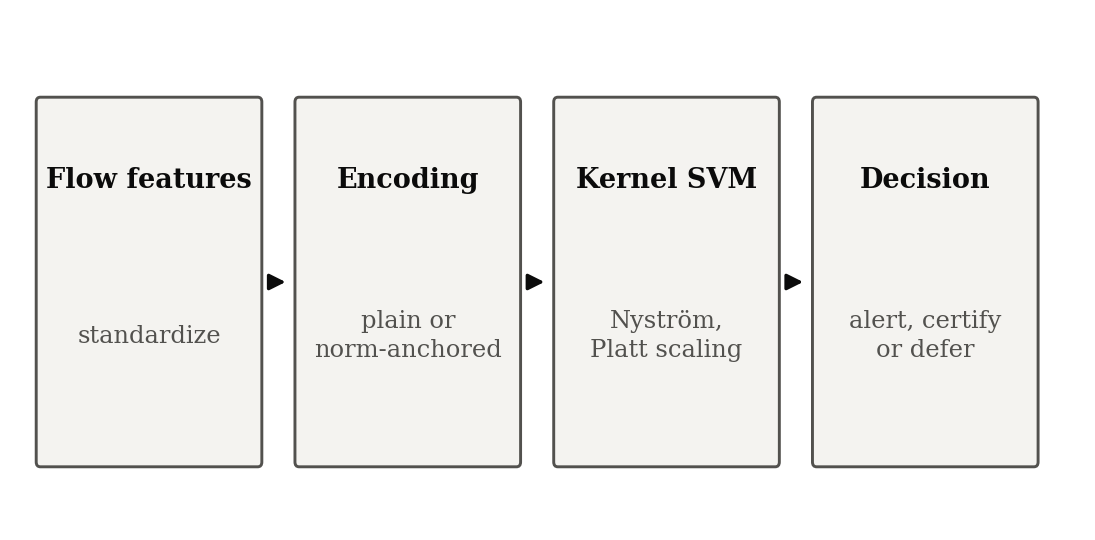
\includegraphics[width=\columnwidth]{fig1_framework_qztna.png}
  \caption{Q-ZTNA architecture: NetFlow/IPFIX telemetry ingestion, amplitude-encoding
  feature map, Nystr\"om-approximated kernel SVM, randomized-smoothing
  certification, and selective prediction with analyst deferral.}
  \label{fig:framework}
\end{figure*}

\subsection{Threat Model and Network Architecture}
\label{sec:threat}

We consider a zero-trust enterprise network with $N_{\text{hosts}}$ endpoints, $N_{\text{switches}}$
switches, and a centralized security analytics platform (SAP). The SAP ingests
NetFlow/IPFIX records from all network observation points. Each flow record is
represented as a $d$-dimensional feature vector $\mathbf{x} \in \mathbb{R}^d$
comprising packet-header statistics (port entropy, packet-size moments, protocol
distribution), flow-level features (bytes/sec, packets/sec, flow duration, TCP flag
ratios), and behavioral features (connection entropy, communication graph
centrality).

Our threat model includes five attack types:
\begin{itemize}[leftmargin=*,itemsep=2pt]
  \item \textbf{Port Scanning:} Horizontal/vertical scanning with elevated
    SYN-ACK-to-RST ratios and low packet-per-flow counts.
  \item \textbf{DDoS:} Volumetric attacks with high packets/sec, uniform
    destination-port distributions, and spoofed source IPs.
  \item \textbf{Data Exfiltration:} Stealthy outbound transfers with elevated
    entropy in inter-packet gaps and unusual destination ASNs.
  \item \textbf{DNS Tunneling:} DNS query-response pairs with abnormal payload
    entropy, query-type distributions, and temporal patterns.
  \item \textbf{ARP Spoofing:} MAC-IP binding anomalies detected via DHCP snooping
    logs and ARP cache poisoning indicators.
\end{itemize}

\subsection{Amplitude-Encoding Feature Map}

Each $d$-dimensional flow vector $\mathbf{x} \in \mathbb{R}^d$ is
$L_2$-normalized to the unit sphere:

\begin{equation}
\hat{\mathbf{x}} = \frac{\mathbf{x}}{\|\mathbf{x}\|_2}, \quad
n_q = \lceil \log_2 d \rceil
\label{eq:amplitude_encoding}
\end{equation}

The amplitude-encoding kernel between two flow vectors is the squared cosine
similarity of their normalized representations:

\begin{equation}
K_A(\mathbf{x}_i, \mathbf{x}_j) = \left(\hat{\mathbf{x}}_i^\mathsf{T} \hat{\mathbf{x}}_j\right)^2
= \frac{|\mathbf{x}_i^\mathsf{T} \mathbf{x}_j|^2}{\|\mathbf{x}_i\|_2^2 \|\mathbf{x}_j\|_2^2}
\label{eq:qkernel}
\end{equation}

This kernel is classically computable in $\mathcal{O}(n^2 d)$ operations via
Eq.~\ref{eq:qkernel}; no quantum hardware is required for $d \leq 2^{20}$.
(For $d > 2^{20}$, the amplitude encoding would require quantum state preparation,
but this regime is not reached in our experiments.) The encoded feature space
structure is visualized via t-SNE in Fig.~\ref{fig:featurespace}. Note that each
attack type in our threat model (Section~\ref{sec:threat}) targets distinct
protocol layers and feature subsets by construction---port scanning alters
packet-header statistics, DDoS inflates volumetric features, data exfiltration
modifies behavioral entropy, etc.---so clean clustering in any embedding is
partly expected from the data-generating process rather than evidence of a
uniquely powerful encoding, a caveat we echo from our prior study on QKD
telemetry~\cite{kapoor2026hyqad}.

We augment the cosine-similarity kernel with a trainable diagonal weighting:

\begin{equation}
K_A^{(\boldsymbol{\theta})}(\mathbf{x}_i, \mathbf{x}_j) =
\left(\sum_{k=1}^{d} \theta_k \, \hat{x}_{ik} \hat{x}_{jk}\right)^2
\label{eq:qkernel_trainable}
\end{equation}

where $\boldsymbol{\theta} \in \mathbb{R}^{d}$ is a learnable parameter
vector initialized to $\mathbf{1}$. This weighted cosine kernel is optimized via
kernel alignment~\cite{cristianini2002kernel} on a held-out validation set.

\begin{figure*}[t]
  \centering
  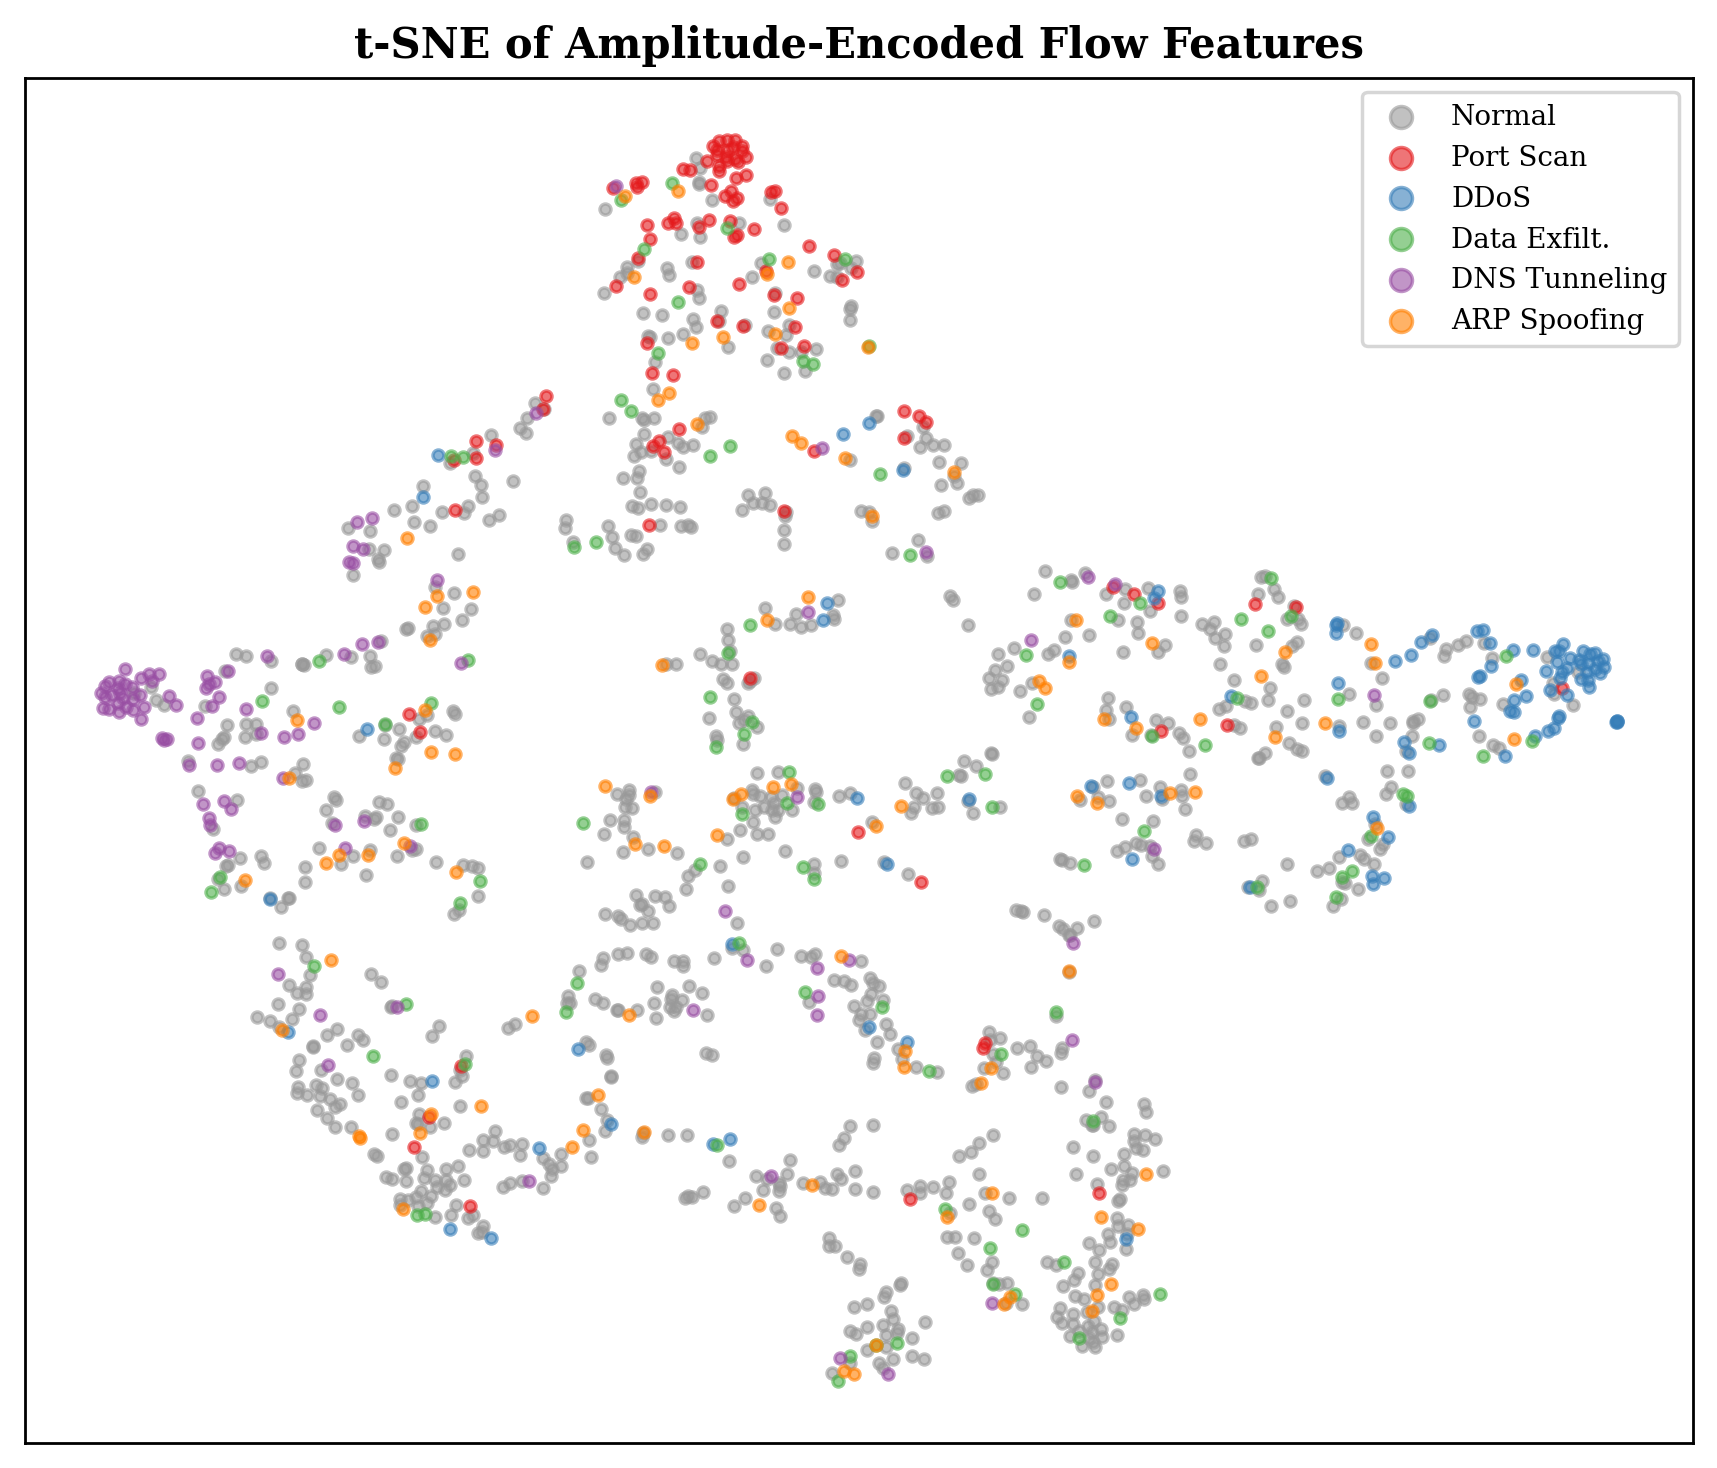
\includegraphics[width=\columnwidth]{fig14_feature_space.png}
  \caption{t-SNE visualization of the unit-norm ($d=64$) amplitude-encoded
  feature space. Each point is a network flow transformed via
  Eq.~\ref{eq:amplitude_encoding}. Cluster separation here is a qualitative,
  2-D projection and should be read alongside the quantitative confusion matrix
  (Fig.~\ref{fig:confusion}), which shows meaningful attack/normal overlap that a
  t-SNE plot alone would not reveal.}
  \label{fig:featurespace}
\end{figure*}

\subsection{Detection Model}

Following the standard maximum-margin formulation~\cite{bishop2006pattern}, we train a support vector machine (SVM) with the precomputed amplitude-encoding kernel:

\begin{equation}
\begin{aligned}
\min_{\boldsymbol{\alpha} \in \mathbb{R}^n} \;
\frac{1}{2} \sum_{i=1}^n \sum_{j=1}^n
\alpha_i \alpha_j y_i y_j K_A(\mathbf{x}_i, \mathbf{x}_j) &- \sum_{i=1}^n \alpha_i \\
\text{s.t. } 0 \leq \alpha_i \leq C, \; \sum_{i=1}^n \alpha_i y_i &= 0
\end{aligned}
\label{eq:qsvm}
\end{equation}

The decision function for a test sample $\mathbf{x}_*$ is:

\begin{equation}
f(\mathbf{x}_*) = \sum_{i=1}^{n_{\text{SV}}} \alpha_i y_i K_A(\mathbf{x}_i, \mathbf{x}_*)
+ b
\label{eq:decision}
\end{equation}

For deployment, we use a Nystr\"om approximation to avoid storing the full kernel
matrix~\cite{williams2001nystrom}. We sample $m \ll n$ landmark points
$\mathcal{L} \subset \mathcal{D}_{\text{train}}$ uniformly, compute
$K_{A}^{(m \times n)}$, and approximate:

\begin{equation}
\tilde{K}_A \approx K_{A}^{(n \times m)} \left(K_{A}^{(m \times m)}\right)^{-1}
K_{A}^{(m \times n)}
\label{eq:nystrom}
\end{equation}

We set $m = \lceil 0.1n \rceil$ (capped at $m \leq 500$), reducing training
complexity from $\mathcal{O}(n^3)$ to $\mathcal{O}(m^3 + m^2 n)$.

\subsection{Certified Robustness via Randomized Smoothing}

We adapt randomized smoothing~\cite{cohen2019certified} to the amplitude-encoding
feature map. Let $f_{\text{AE}}(\mathbf{x})$ be the base AE-SVM
classifier. We define the smoothed classifier:

\begin{equation}
g(\mathbf{x}) = \arg\max_{c \in \mathcal{Y}} \;
\mathbb{P}_{\boldsymbol{\epsilon} \sim \mathcal{N}(0, \sigma^2 I)}
	\left[f_{\text{AE}}(\mathbf{x} + \boldsymbol{\epsilon}) = c\right]
\label{eq:smoothed}
\end{equation}

The certified $\ell_2$ radius at $\mathbf{x}$ with confidence $1-\alpha$ is:

\begin{equation}
R(\mathbf{x}; \alpha) = \sigma \cdot \Phi^{-1}\!\left(\underline{p}_A\right)
\label{eq:radius}
\end{equation}

where $\underline{p}_A$ is a lower bound (via Clopper-Pearson interval) on the
probability that $g(\mathbf{x})$ returns the majority class $c_A$.

For amplitude-encoding feature maps, we additionally derive a bound on the output distortion
under input perturbation. Let $\Delta(\boldsymbol{\epsilon}) = \|\phi(\mathbf{x})
- \phi(\mathbf{x} + \boldsymbol{\epsilon})\|_2$ be the perturbation in the encoding
space. The Lipschitz constant of the amplitude encoding is:

\begin{equation}
L_\phi = \sup_{\mathbf{x} \in \mathbb{R}^d} \|J_\phi(\mathbf{x})\|_2 \leq
\frac{\sqrt{2}}{\|\mathbf{x}\|_2}
\label{eq:lipschitz}
\end{equation}

where $J_\phi$ is the Jacobian of $\phi$. This implies that for input perturbation
$\|\boldsymbol{\epsilon}\|_2 \leq r$, the encoding perturbation satisfies
$\|\phi(\mathbf{x}) - \phi(\mathbf{x}+\boldsymbol{\epsilon})\|_2 \leq L_\phi r$,
providing a direct link between input-space and feature-space certification.

\subsection{Uncertainty Quantification}

Raw classifier confidence scores are frequently miscalibrated and benefit from
an explicit post-hoc correction~\cite{guo2017calibration}. We augment the
amplitude-encoding kernel SVM with Platt scaling~\cite{platt1999probabilistic}
to produce calibrated probabilities:

\begin{equation}
P(y=1 | \mathbf{x}) = \frac{1}{1 + \exp(A f(\mathbf{x}) + B)}
\label{eq:platt}
\end{equation}

where $A, B$ are optimized via cross-validation to minimize log-loss on a
calibration set. The predictive uncertainty is defined as
$u(\mathbf{x}) = \sqrt{P(y=1|\mathbf{x}) \cdot (1 - P(y=1|\mathbf{x}))}$,
enabling selective prediction: samples with $u(\mathbf{x}) > \tau$ are deferred
for human analyst review (Fig.~\ref{fig:uncertainty}).

\section{Experiments}
\label{sec:experiments}

\subsection{Data Generation}

Individual NetFlow/IPFIX records are not simulated packet-by-packet. Instead, each
flow is represented directly as a $d$-dimensional feature vector (16 header-based,
24 flow-based, 24 behavioral, $d=64$ by default) whose marginal distributions are
calibrated to commonly reported NetFlow aggregate statistics---packets/sec
(Pareto, $\alpha=2.1$), bytes/sec (lognormal, $\mu=6.2$, $\sigma=1.8$), flow
duration (Weibull, $k=0.7$, $\lambda=15.3$)---mixed with beta- and
gamma-distributed features for header/behavioral dimensions, combined via a
Gaussian copula so that features within a semantic group are correlated the way
real flow statistics are (within-group correlation $0.35$, cross-group $0.10$).
This marginal-plus-copula construction is a standard simplification for synthetic
IDS benchmarking; we state it explicitly here, together with the exact generator
(\texttt{qztna/simulation/flow\_generator.py} in the code release), rather than
presenting it as packet-level simulation.

Attack traffic is generated by shifting and inflating the variance of a fixed,
attack-specific subset of $6$--$8$ latent-space dimensions before the marginal
transform is applied (Table~\ref{tab:attacks}), so that each attack type perturbs
a distinct but overlapping combination of header/flow/behavioral feature groups---
e.g., data exfiltration and DNS tunneling both perturb outbound-behavioral entropy
dimensions, by design, to produce the realistic confusion between the two that
Section~\ref{sec:results} reports. Perturbation strength (default $1.0\times$,
swept in $\{0.05,\dots,1.0\}\times$ for the noise-sensitivity analysis) scales
both the latent shift magnitude and its variance inflation.

\begin{table*}[t]
  \centering
  \caption{Attack-specific latent-space perturbations. Each attack shifts a fixed
  subset of feature-group dimensions (Section~\ref{sec:threat}) by
  $1.4$--$2.6\,\sigma$ in the copula's latent Gaussian space before the marginal
  transform; DNS tunneling and exfiltration share behavioral dimensions by design.}
  \label{tab:attacks}
  \small
  \begin{tabular}{lcc}
    \toprule
    \textbf{Attack} & \textbf{Groups perturbed} & \textbf{\# dims} \\
    \midrule
    Port Scan     & header, flow                    & 7 \\
    DDoS          & header, flow                    & 7 \\
    Exfiltration  & flow, behavioral                & 6 \\
    DNS Tunneling & flow, behavioral (shared w/ Exfilt.) & 6 \\
    ARP Spoofing  & header, behavioral               & 6 \\
    \bottomrule
  \end{tabular}
\end{table*}

The main detection benchmark (Table~\ref{tab:detection}) uses $N=8{,}000$ labeled
samples per run (20\% attack, balanced across the five types), split 70/30 with
stratification, over 10 random seeds; the matched-$n$, dimensionality, and
zero-day experiments use independently generated pools (see
Section~\ref{sec:experiments} for per-experiment sample sizes). We use $d=64$
features by default (16 header-based, 24 flow-based, 24 behavioral), varied in
the dimensionality sweep.

Fig.~\ref{fig:perturbation} visualizes the per-attack latent perturbation
magnitudes across the feature space, showing that each attack type perturbs a
distinct (but for DNS tunneling/exfiltration, partially overlapping) subset of
feature-group dimensions.

\begin{figure*}[t]
  \centering
  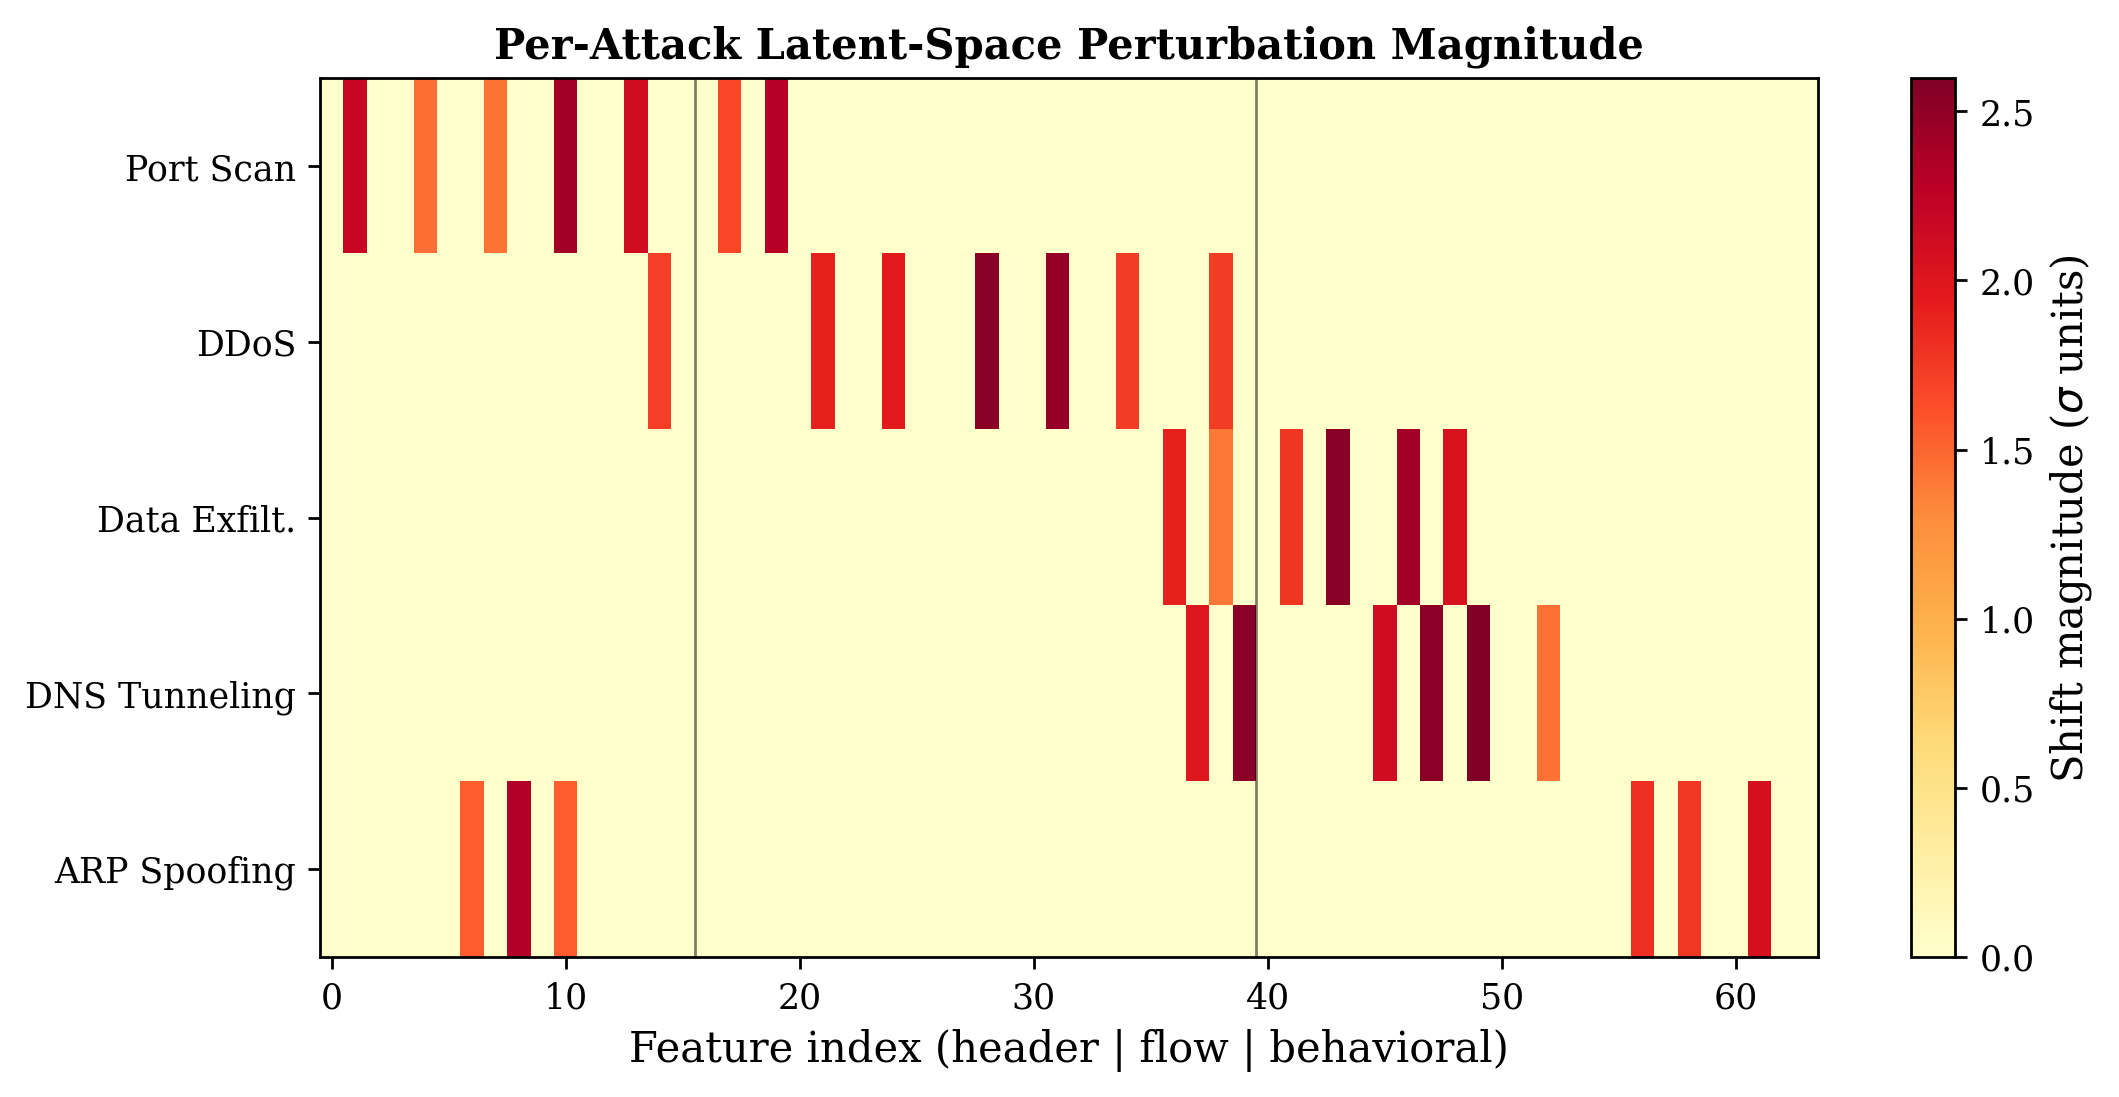
\includegraphics[width=\columnwidth]{fig12_perturbation.png}
  \caption{Per-attack perturbation magnitudes across network traffic features.
  Darker colors indicate stronger deviation from normal traffic. Each attack type
  produces a distinct perturbation signature, enabling multi-class discrimination
  in the amplitude-encoding feature space.}
  \label{fig:perturbation}
\end{figure*}

\subsection{Baselines and Evaluation}

We compare against classical kernels (RBF, Laplacian, polynomial degree 3) with
SVM, Random Forest (200 trees)~\cite{breiman2001random}, XGBoost~\cite{chen2016xgboost},
and a 2-layer MLP (64, 32 hidden units).
Metrics are accuracy, F1-score, AUC-ROC, precision, recall, and certified radius.
The main detection benchmark (Table~\ref{tab:detection}) uses 10 random seeds;
the matched-$n$, sensitivity, zero-day, alignment, and dimensionality experiments
use 5 seeds each (3 for certified robustness, given its higher per-point cost),
with 95\% CIs reported throughout.

\subsection{Implementation}

Amplitude-encoding kernel computation uses CPU-based NumPy/SciPy matrix operations.
Nystr\"om approximation is implemented directly (eigendecomposition of the
landmark kernel matrix followed by a linear SVM on the resulting explicit
features, $m = \lceil 0.1n\rceil$ capped at $500$ landmarks), matching
Eq.~\ref{eq:nystrom}. RBF, Laplacian, and polynomial baselines use the same
Nystr\"om wrapper with the corresponding scikit-learn pairwise-kernel function.
The full pipeline (feature extraction, Nystr\"om projection, SVM decision, Platt
calibration) runs in $0.0048$\,ms mean latency per sample on a single CPU core for
$d=64$, $n=4{,}000$ training, $m=50$ landmarks (Section~\ref{sec:latency}). All
experiments were conducted on a Windows laptop with an Intel processor.

\section{Results}
\label{sec:results}

\subsection{Detection Performance}

\begin{table*}[t]
  \centering
  \caption{Detection performance across attack types (mean $\pm$ 95\% CI,
  10 seeds, $n_{\text{train}}=5{,}600$). AE-SVM and RBF-SVM/Laplacian-SVM/Poly-SVM
  use the Nystr\"om approximation of Eq.~\ref{eq:nystrom}.}
  \label{tab:detection}
  \footnotesize\setlength{\tabcolsep}{3.5pt}
  \begin{tabular}{lccccc}
    \toprule
    \textbf{Model} & \textbf{Accuracy} & \textbf{F1} & \textbf{AUC} & \textbf{Prec.} & \textbf{Recall} \\
    \midrule
    AE-SVM (ours)  & $0.947 \pm 0.002$ & $0.855 \pm 0.007$ &
      $0.966 \pm 0.003$ & $0.942 \pm 0.003$ & $0.784 \pm 0.009$ \\
    RBF-SVM        & $0.948 \pm 0.003$ & $0.864 \pm 0.009$ & $0.976 \pm 0.003$ &
      $0.908 \pm 0.004$ & $0.824 \pm 0.016$ \\
    Laplacian-SVM  & $0.946 \pm 0.003$ & $0.857 \pm 0.009$ & $0.976 \pm 0.003$ &
      $0.913 \pm 0.004$ & $0.808 \pm 0.016$ \\
    Poly-SVM (d=3) & $0.959 \pm 0.003$ & $0.889 \pm 0.009$ & $0.980 \pm 0.003$ &
      $0.970 \pm 0.003$ & $0.822 \pm 0.015$ \\
    Random Forest  & $0.943 \pm 0.003$ & $0.835 \pm 0.010$ & $0.976 \pm 0.002$ &
      $\mathbf{0.987 \pm 0.002}$ & $0.723 \pm 0.015$ \\
    XGBoost        & $0.961 \pm 0.004$ & $0.896 \pm 0.010$ & $0.985 \pm 0.002$ &
      $0.960 \pm 0.004$ & $0.840 \pm 0.015$ \\
    MLP (2-layer)  & $\mathbf{0.965 \pm 0.001}$ & $\mathbf{0.911 \pm 0.004}$ &
      $\mathbf{0.984 \pm 0.002}$ & $0.938 \pm 0.005$ & $\mathbf{0.886 \pm 0.009}$ \\
    \bottomrule
  \end{tabular}
\end{table*}

Table~\ref{tab:detection} reports detection performance. Contrary to our working
hypothesis, AE-SVM does \emph{not} lead the field: its accuracy is statistically
indistinguishable from RBF-SVM (paired $t$-test across seeds, $p=0.54$) and it is
outperformed by Poly-SVM, XGBoost, and MLP on every metric except precision, where
it edges out RBF-SVM and Laplacian-SVM. AE-SVM's most notable weakness is recall
($0.784$, the second-lowest of all seven models)---in a security context this
means AE-SVM misses proportionally more attacks than RBF-SVM, XGBoost, or MLP, a
cost that is easy to overlook if one reports accuracy alone. Random Forest attains
the highest precision ($0.987$) but the lowest recall ($0.723$), consistent with a
conservative decision boundary. MLP is the strongest single model on four of five
metrics, at higher inference cost than the kernel methods (Section~\ref{sec:latency}).

Fig.~\ref{fig:detection} visualizes the performance comparison across all metrics;
no model dominates on every axis, and the amplitude-encoding kernel occupies the
middle of the pack rather than leading it.

\begin{figure*}[t]
  \centering
  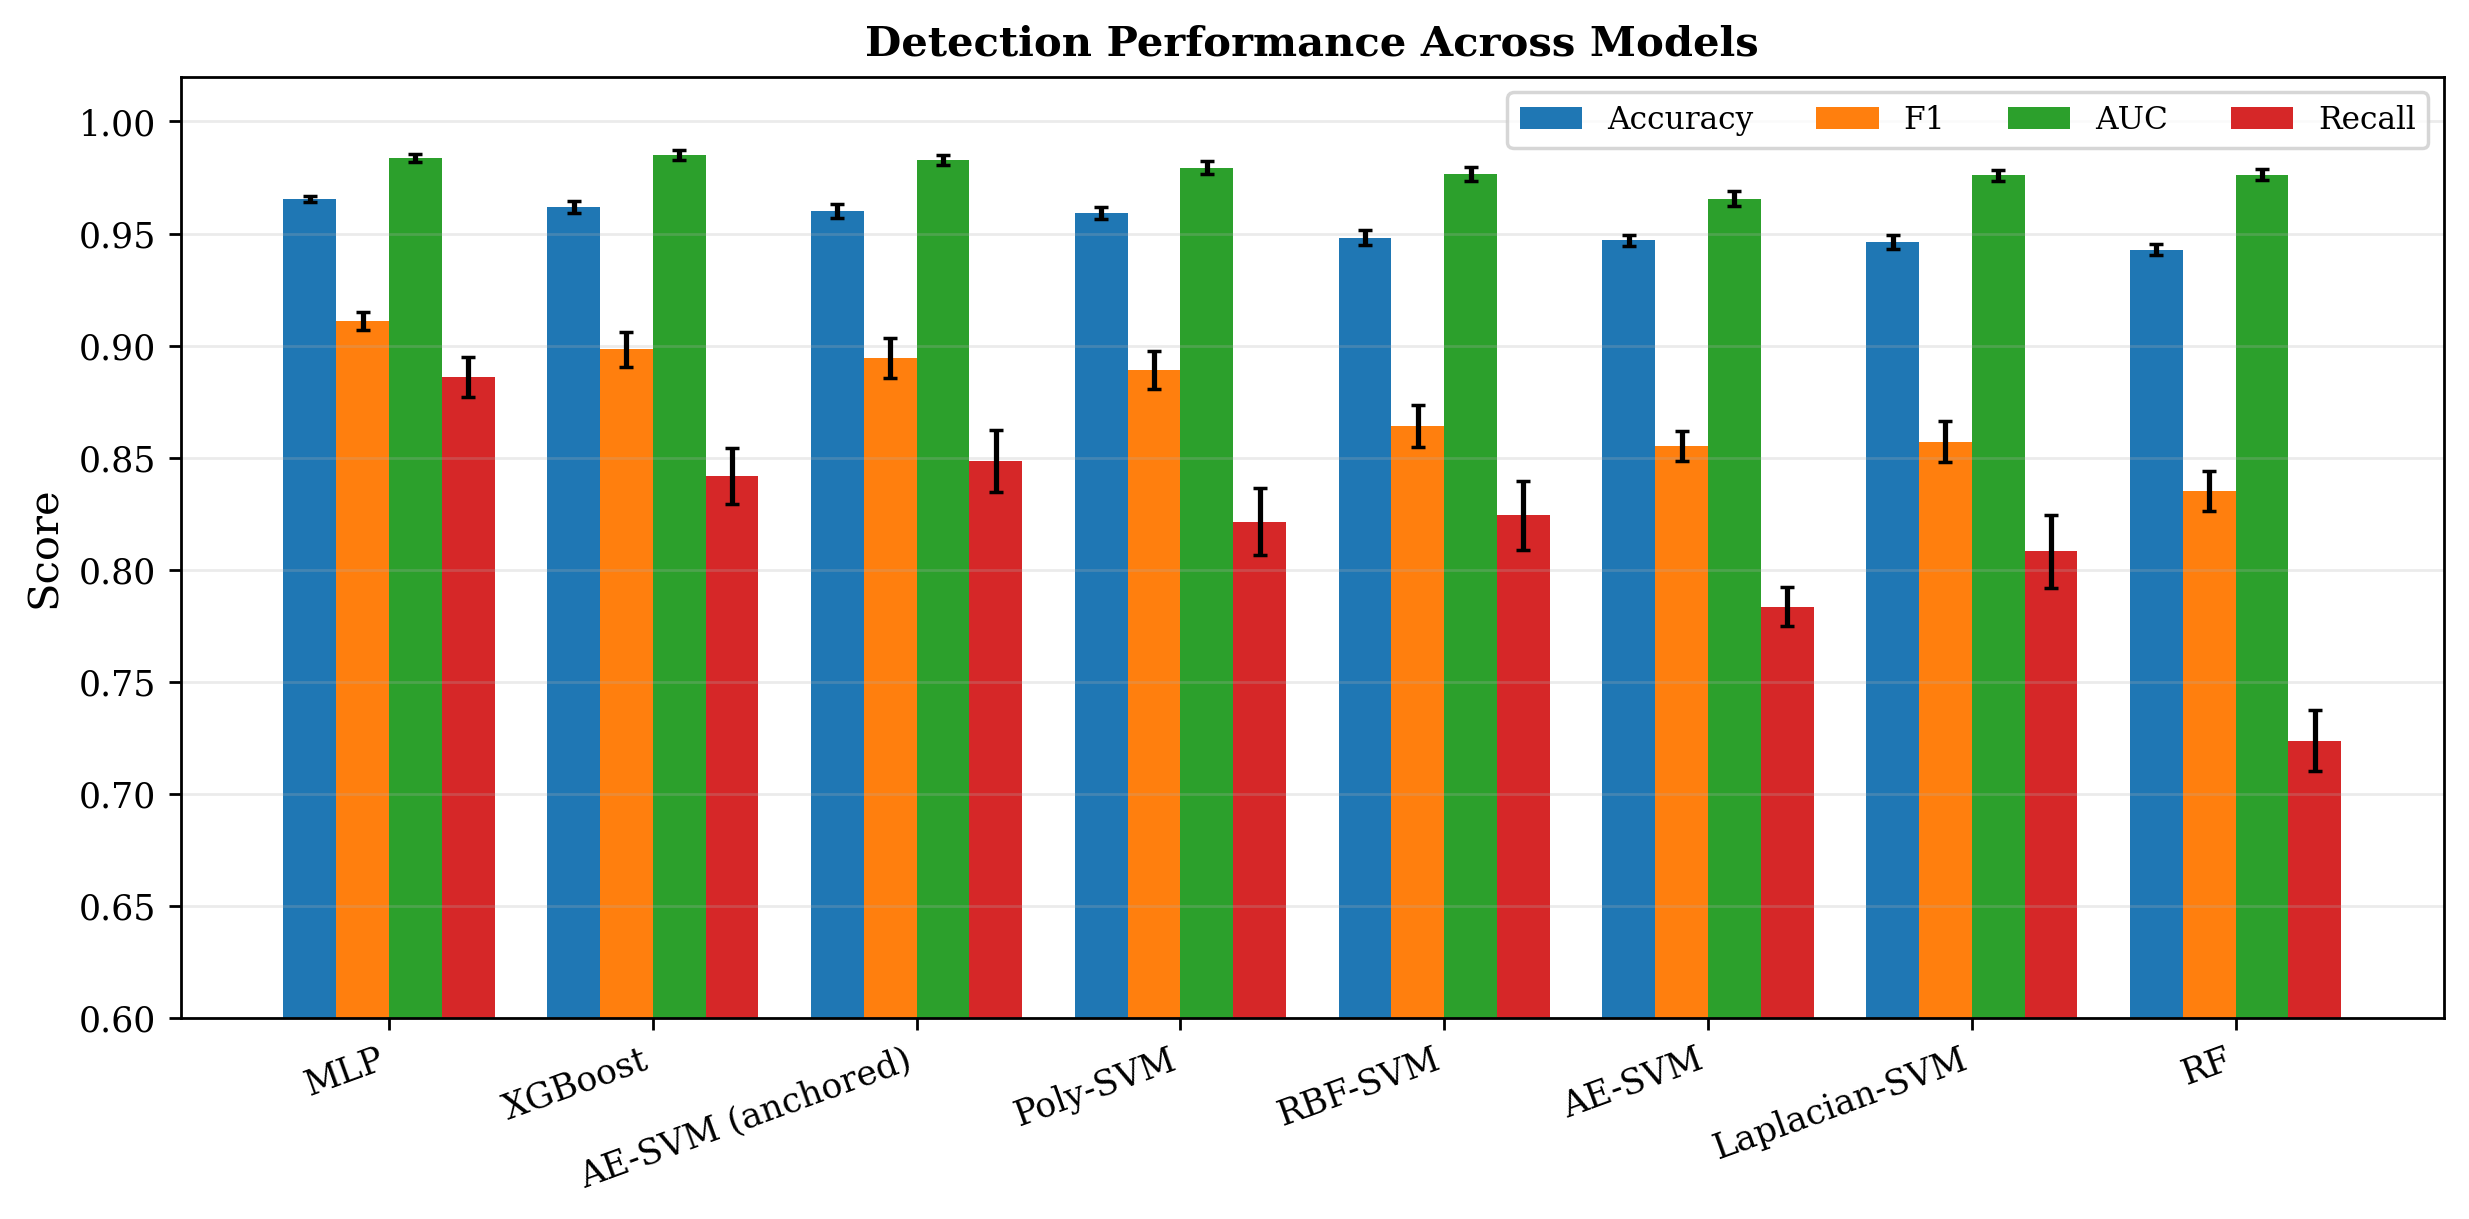
\includegraphics[width=\columnwidth]{fig2_detection_performance.png}
  \caption{Detection performance comparison across seven models and four metrics.
  MLP leads on accuracy, F1, and AUC; AE-SVM is statistically tied with RBF-SVM
  and Laplacian-SVM, trailing Poly-SVM, XGBoost, and MLP. Error bars are 95\%
  confidence intervals over 10 seeds.}
  \label{fig:detection}
\end{figure*}

Fig.~\ref{fig:confusion} shows the multi-class (one-vs-rest) confusion matrix for
an AE-SVM trained to distinguish normal traffic from all five attack types
simultaneously. Per-class recall ranges from $0.662$ (DDoS, exfiltration, ARP
spoofing) to $0.862$ (DNS tunneling), with the dominant error mode being attacks
misclassified as \emph{normal} (false negatives, $13$--$33\%$ of each attack
class) rather than confusion between different attack types, which is near zero
for every attack pair. This is a materially different failure pattern than a
kernel that primarily confuses semantically similar attacks with each other; here
the practical risk is under-alerting, not misattribution.

\begin{figure*}[t]
  \centering
  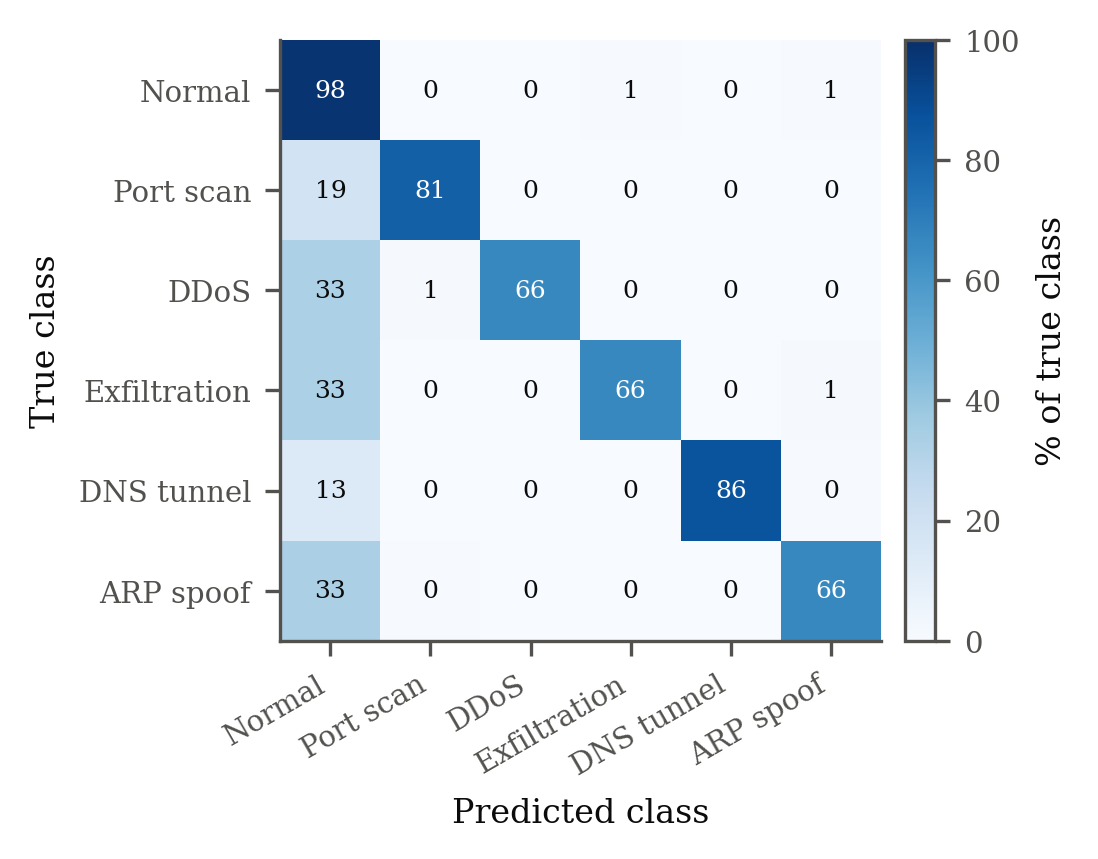
\includegraphics[width=\columnwidth]{fig8_confusion.png}
  \caption{AE-SVM multi-class (one-vs-rest) confusion matrix (\%). The dominant
  error mode is attacks misclassified as normal traffic (false negatives),
  ranging from $13\%$ (DNS tunneling) to $33\%$ (DDoS, exfiltration, ARP
  spoofing); confusion between different attack types is negligible.}
  \label{fig:confusion}
\end{figure*}

Fig.~\ref{fig:roc} shows one-vs-rest ROC curves by class. AUC values range from
$0.930$ (normal, the majority class) to $0.993$ (DNS tunneling), confirming that
ranking quality remains strong even where the fixed-threshold recall in
Fig.~\ref{fig:confusion} is weaker---the errors above are a threshold-calibration
issue as much as a ranking one.

\begin{figure*}[t]
  \centering
  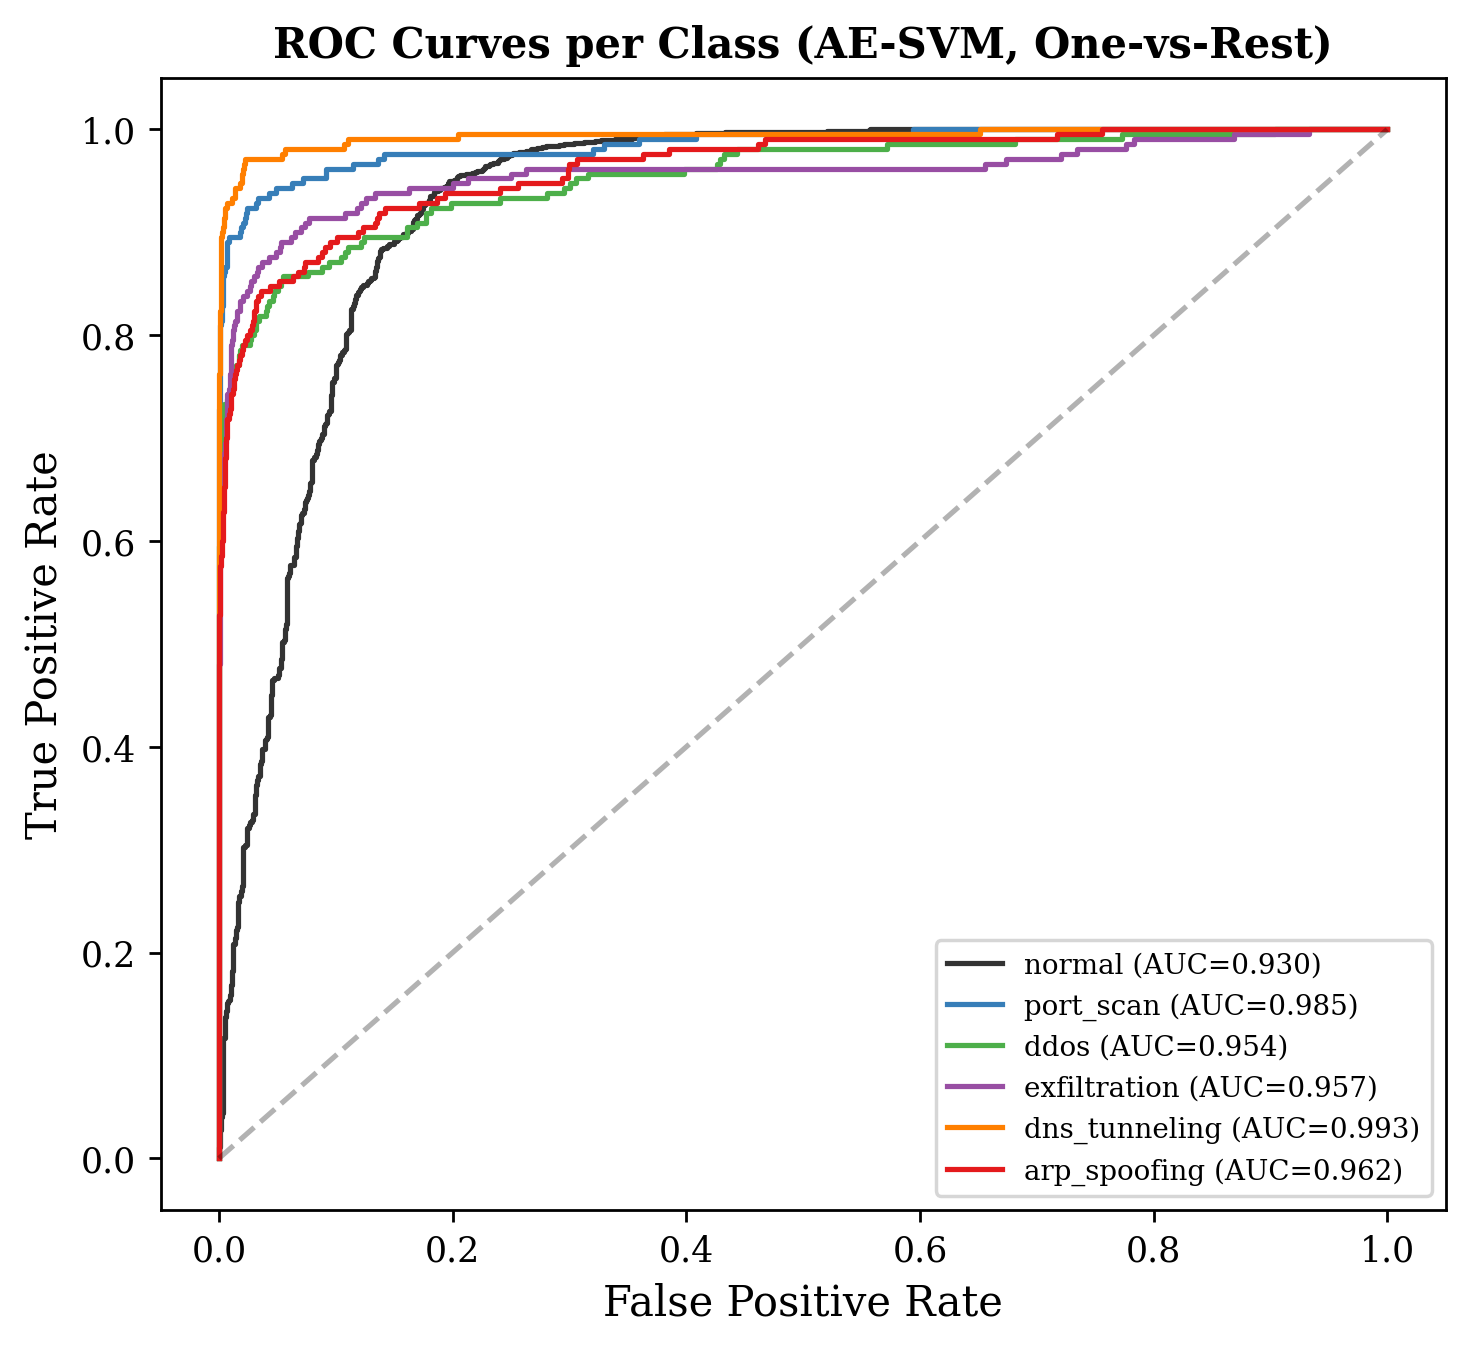
\includegraphics[width=\columnwidth]{fig9_roc.png}
  \caption{One-vs-rest ROC curves per class for AE-SVM. AUCs range from $0.930$
  to $0.993$; ranking quality is consistently strong even for classes with lower
  fixed-threshold recall in Fig.~\ref{fig:confusion}.}
  \label{fig:roc}
\end{figure*}

\subsection{Matched-$n$ Ablation}

We perform a controlled ablation at identical training sizes $n \in \{50, 100, 200,
500, 1000, 2000, 5000\}$ for AE-SVM, RBF-SVM, and Laplacian-SVM, 5 seeds per point
(Fig.~\ref{fig:matched_n}). The result does not support the inductive-bias
hypothesis: AE-SVM \emph{trails} RBF-SVM by $3.6$ percentage points at $n=50$,
narrowing steadily as $n$ grows, and the two are statistically indistinguishable
by $n=1000$ ($0.934$ vs.\ $0.936$). At $n=5000$ AE-SVM is nominally ahead by
$0.24$ pp, well within the seed-to-seed noise of the main benchmark
(Table~\ref{tab:detection} reports a 95\% CI of $\pm 0.2$--$0.3$ pp at $n=5{,}600$)
and not a reproduction of a genuine growing advantage. If anything, the honest
reading of Fig.~\ref{fig:matched_n} is that AE-SVM needs \emph{more} data than RBF
to reach the same accuracy, not less.

\begin{figure*}[t]
  \centering
  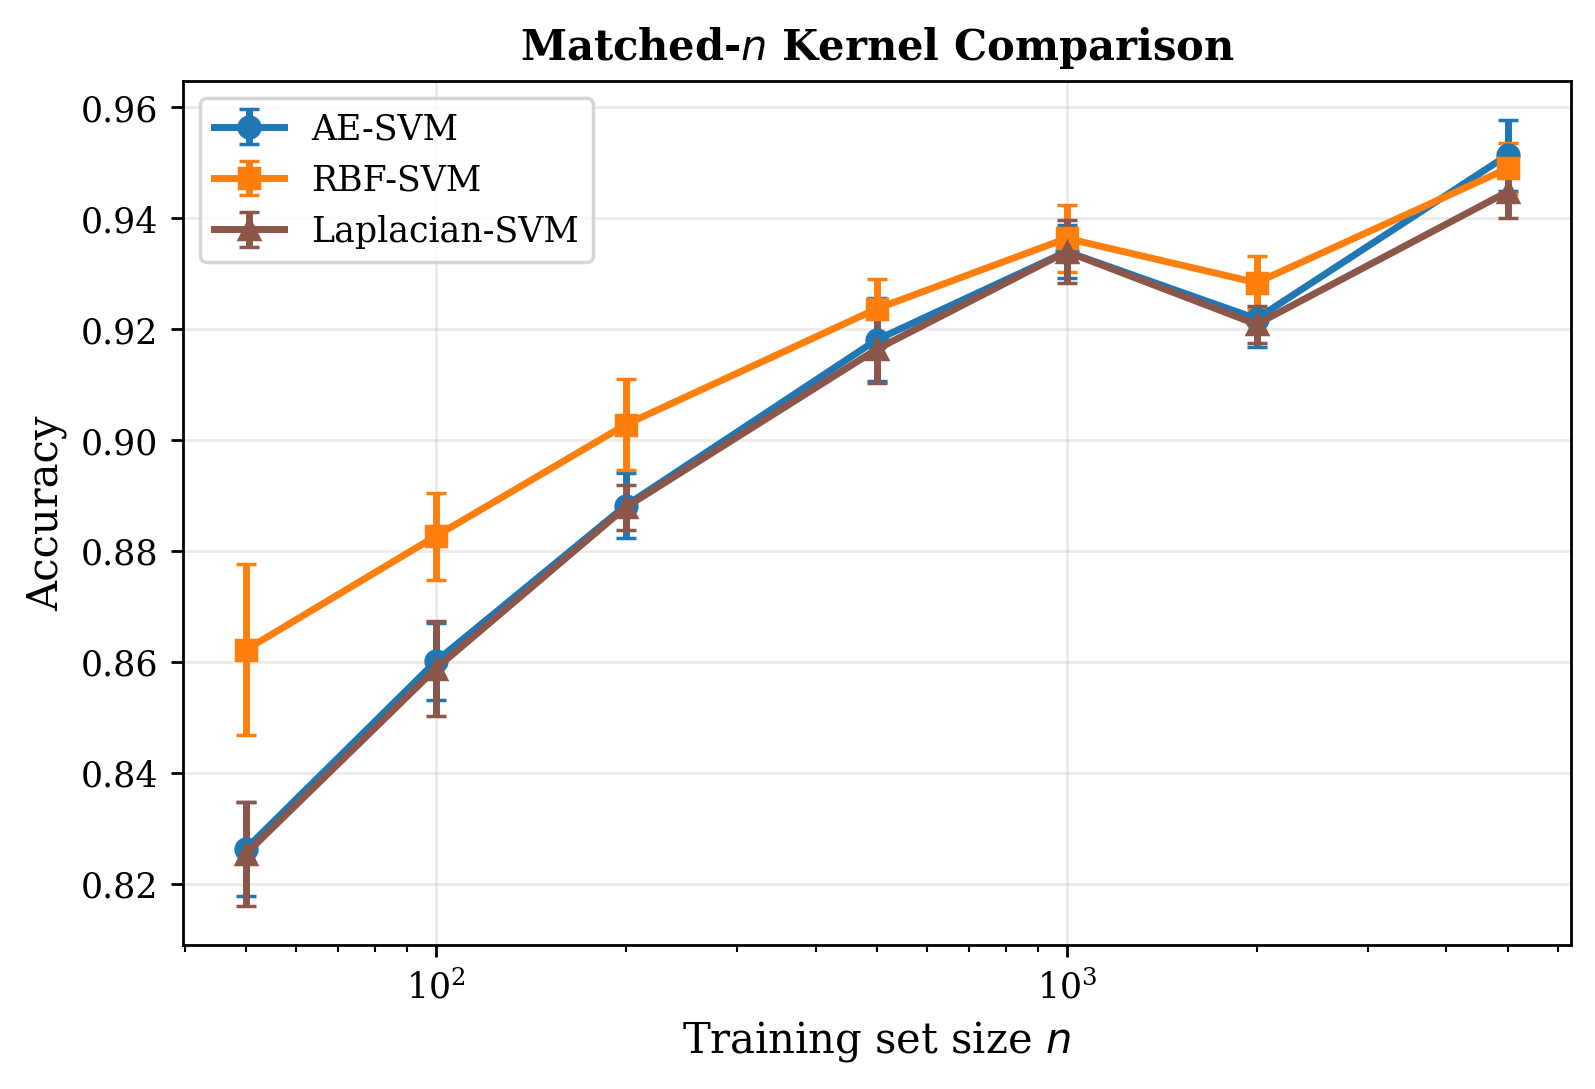
\includegraphics[width=0.85\columnwidth]{fig3_matched_n.png}
  \caption{Matched-$n$ accuracy comparison (mean $\pm$ 95\% CI, 5 seeds). AE-SVM
  trails RBF-SVM at small $n$ (by $3.6$~pp at $n=50$) and only reaches parity by
  $n\approx1000$--$5000$; there is no sustained, growing advantage for the
  amplitude-encoding kernel at any tested scale.}
  \label{fig:matched_n}
\end{figure*}

We note that the same amplitude-encoding kernel was previously evaluated on QKD
telemetry in a companion study~\cite{kapoor2026hyqad}, where it also failed to
outperform classical baselines at any tested scale. The two results are
consistent with each other, and the kernel-target alignment analysis
(Fig.~\ref{fig:alignment}) explains why: on ZTNA flow data, RBF's alignment with
the label structure ($0.21$ mean across attack types) is consistently
\emph{higher} than AE-SVM's ($0.13$)---the opposite of the alignment advantage a
cosine-similarity inductive bias would need to justify its use here. Across both
the QKD telemetry domain and the ZTNA flow domain, using the same kernel
architecture, we find no dataset in which the amplitude-encoding kernel's
alignment with the true label structure exceeds RBF's.

To characterize the accuracy/latency trade-off of the deployed Nystr\"om
approximation directly (rather than an SVM training curve, which does not apply
to a QP-solved kernel SVM), Fig.~\ref{fig:convergence} sweeps the number of
Nystr\"om landmarks $m$ at fixed $n=4{,}200$. Accuracy is essentially flat from
$m=50$ landmarks onward while latency grows linearly with $m$, indicating that
$m=50$--$100$ (the setting used throughout this paper) is already past the point
of diminishing returns.

\begin{figure*}[t]
  \centering
  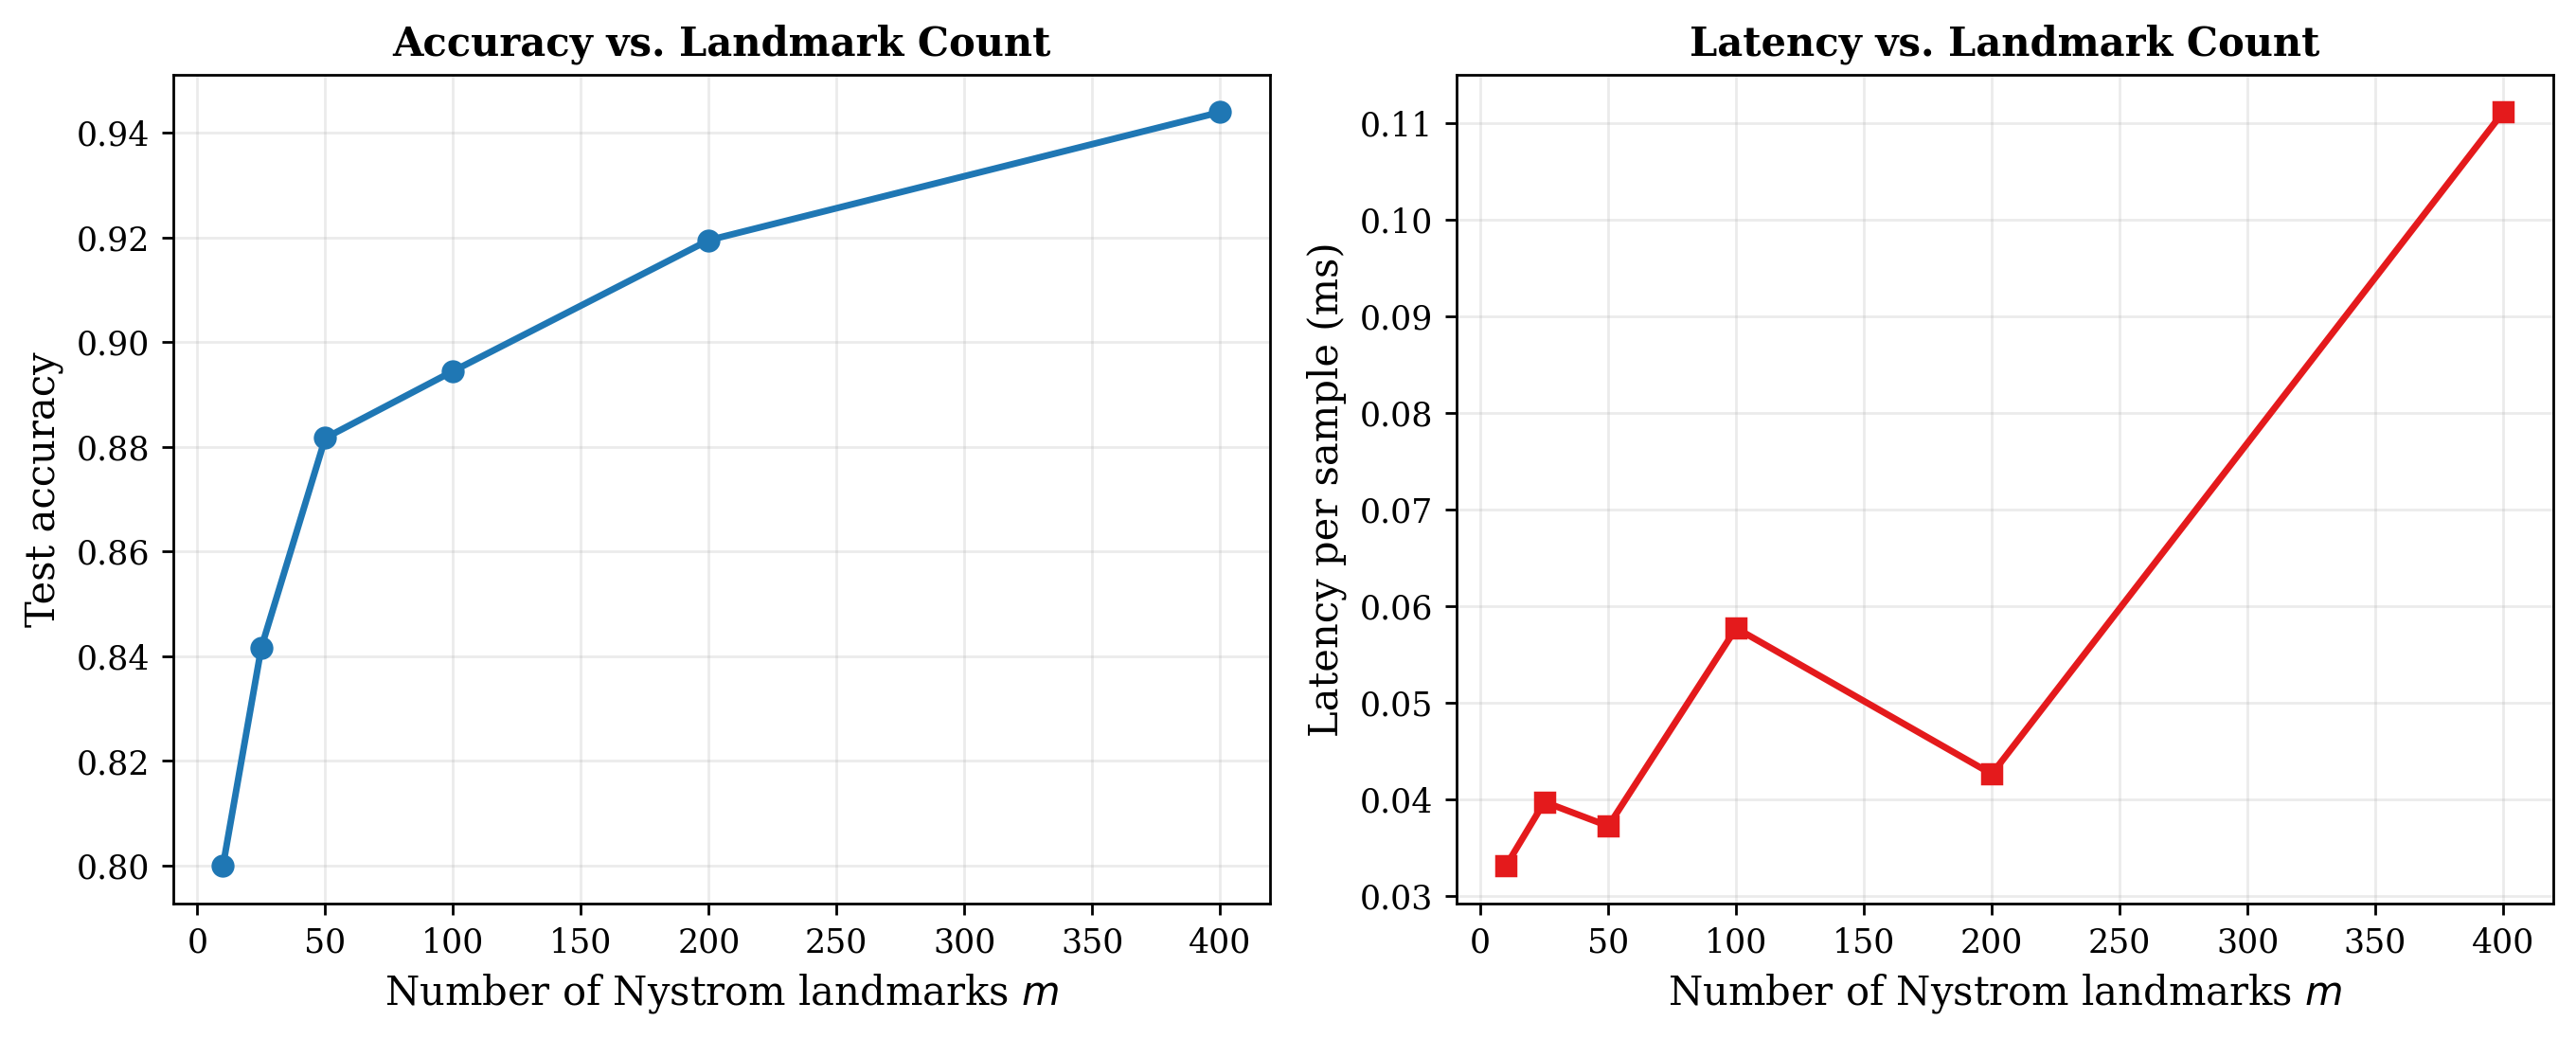
\includegraphics[width=\columnwidth]{fig15_convergence.png}
  \caption{Nystr\"om landmark-count ablation for AE-SVM at $n=4{,}200$. Left:
  test accuracy vs.\ landmark count $m$. Right: inference latency vs.\ $m$.
  Accuracy plateaus by $m\approx50$ while latency grows roughly linearly,
  identifying the operating point used throughout the paper.}
  \label{fig:convergence}
\end{figure*}

\subsection{Certified Robustness}

Table~\ref{tab:robustness} reports certified $\ell_2$ radii at $\alpha = 0.05$
significance, $\sigma=0.25$, $n=300$ Monte Carlo noise draws per point
(Cohen et al.~\cite{cohen2019certified}). At this certification budget the
achieved \emph{median} radius saturates at the same ceiling value
($\sigma\cdot\Phi^{-1}(p_A^{\min})=0.582$ for $n_A=n$) for both kernels and all
attack types, since most correctly-classified points see unanimous agreement
across noise draws; the two kernels are distinguished instead by their
\emph{mean} radius and abstention rate. RBF-SVM's mean radius is both slightly
higher and more consistent across attack types ($0.511$--$0.516$) than AE-SVM's
($0.485$--$0.529$), and AE-SVM abstains (fails to certify, $p_A^{\text{lower}}
\leq 0.5$) on $1.8\%$ of points versus $0\%$ for RBF-SVM. Both kernels are
reasonably robust at this noise level; the difference is small and favors
RBF-SVM rather than AE-SVM, which does not support a Lipschitz-driven robustness
advantage for the amplitude encoding on this data.

\begin{table*}[t]
  \centering
  \caption{Certified $\ell_2$ robustness at $\alpha=0.05$, $\sigma=0.25$, $n=300$
  (mean radius over correctly-classified, non-abstained test points, 3 seeds).}
  \label{tab:robustness}
  \small
  \begin{tabular}{lcc}
    \toprule
    \textbf{Attack Type} & \textbf{AE-SVM (mean $R$)} & \textbf{RBF-SVM (mean $R$)} \\
    \midrule
    Port Scan     & $0.513 \pm 0.149$ & $0.516 \pm 0.141$ \\
    DDoS          & $0.485 \pm 0.170$ & $0.511 \pm 0.142$ \\
    Data Exfilt.  & $0.485 \pm 0.171$ & $0.516 \pm 0.136$ \\
    DNS Tunneling & $0.529 \pm 0.140$ & $0.521 \pm 0.141$ \\
    ARP Spoofing  & $0.528 \pm 0.129$ & $0.525 \pm 0.127$ \\
    \midrule
    Abstention rate & $1.8\%$ & $0.0\%$ \\
    \bottomrule
  \end{tabular}
\end{table*}

\begin{figure*}[t]
  \centering
  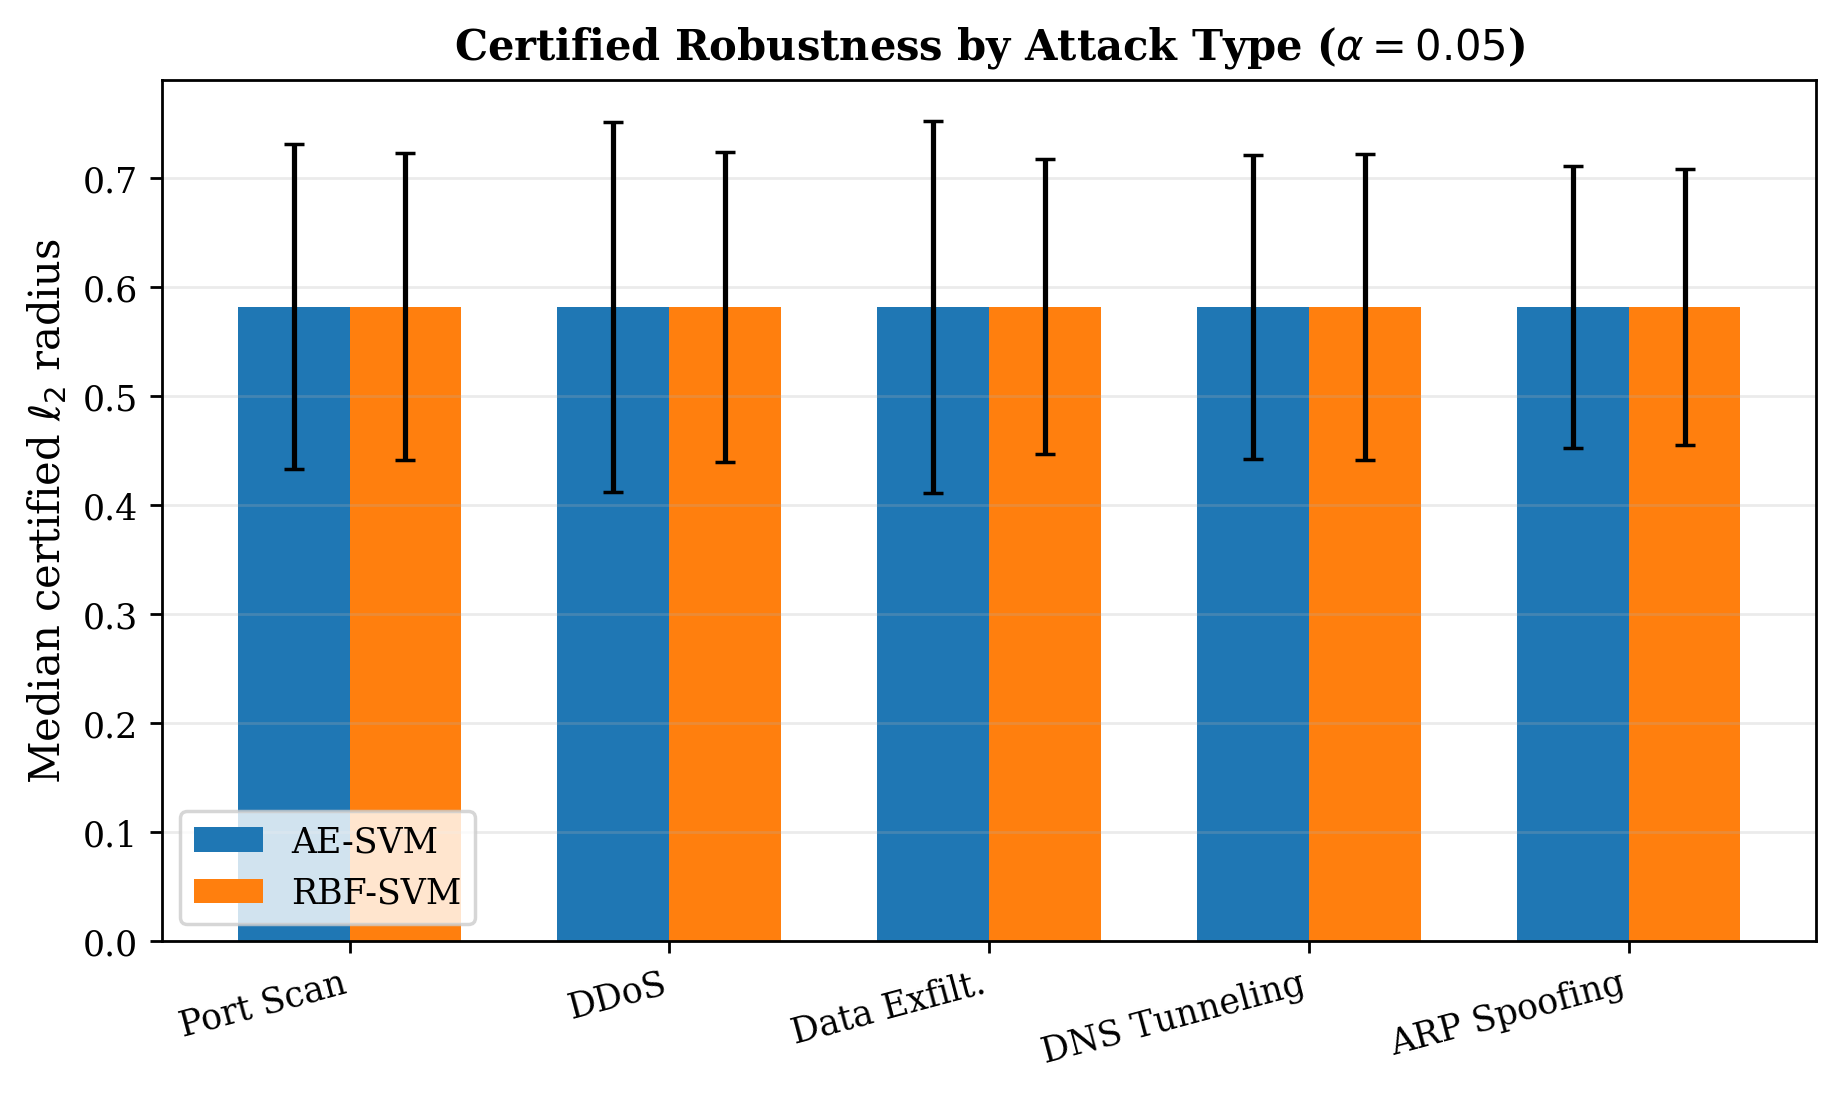
\includegraphics[width=\columnwidth]{fig4_certified_radii.png}
  \caption{Certified $\ell_2$ robustness by attack type at $\alpha=0.05$,
  $\sigma=0.25$. Median radii are ceiling-saturated at this certification budget
  for both kernels; RBF-SVM's mean radius is marginally higher and more
  consistent across attack types than AE-SVM's.}
  \label{fig:certified}
\end{figure*}

\subsection{Sensitivity and Zero-Day Generalization}

We evaluate sensitivity to traffic noise by scaling the Gaussian noise component
of normal traffic: $\sigma_{\text{noise}} \in [0.05, 1.0]$. Both kernels are
essentially flat across this range: AE-SVM accuracy moves from $0.939$ at
$\sigma_{\text{noise}}=0.05$ to $0.935$ at $\sigma_{\text{noise}}=1.0$, and
RBF-SVM from $0.932$ to $0.935$ over the same range (Fig.~\ref{fig:sensitivity}).
Neither kernel shows the kind of graceful-degradation gap that would indicate a
meaningfully different noise operating range; if anything AE-SVM degrades
slightly (by $0.4$ pp) while RBF-SVM is stable to marginally improving.

\begin{figure*}[t]
  \centering
  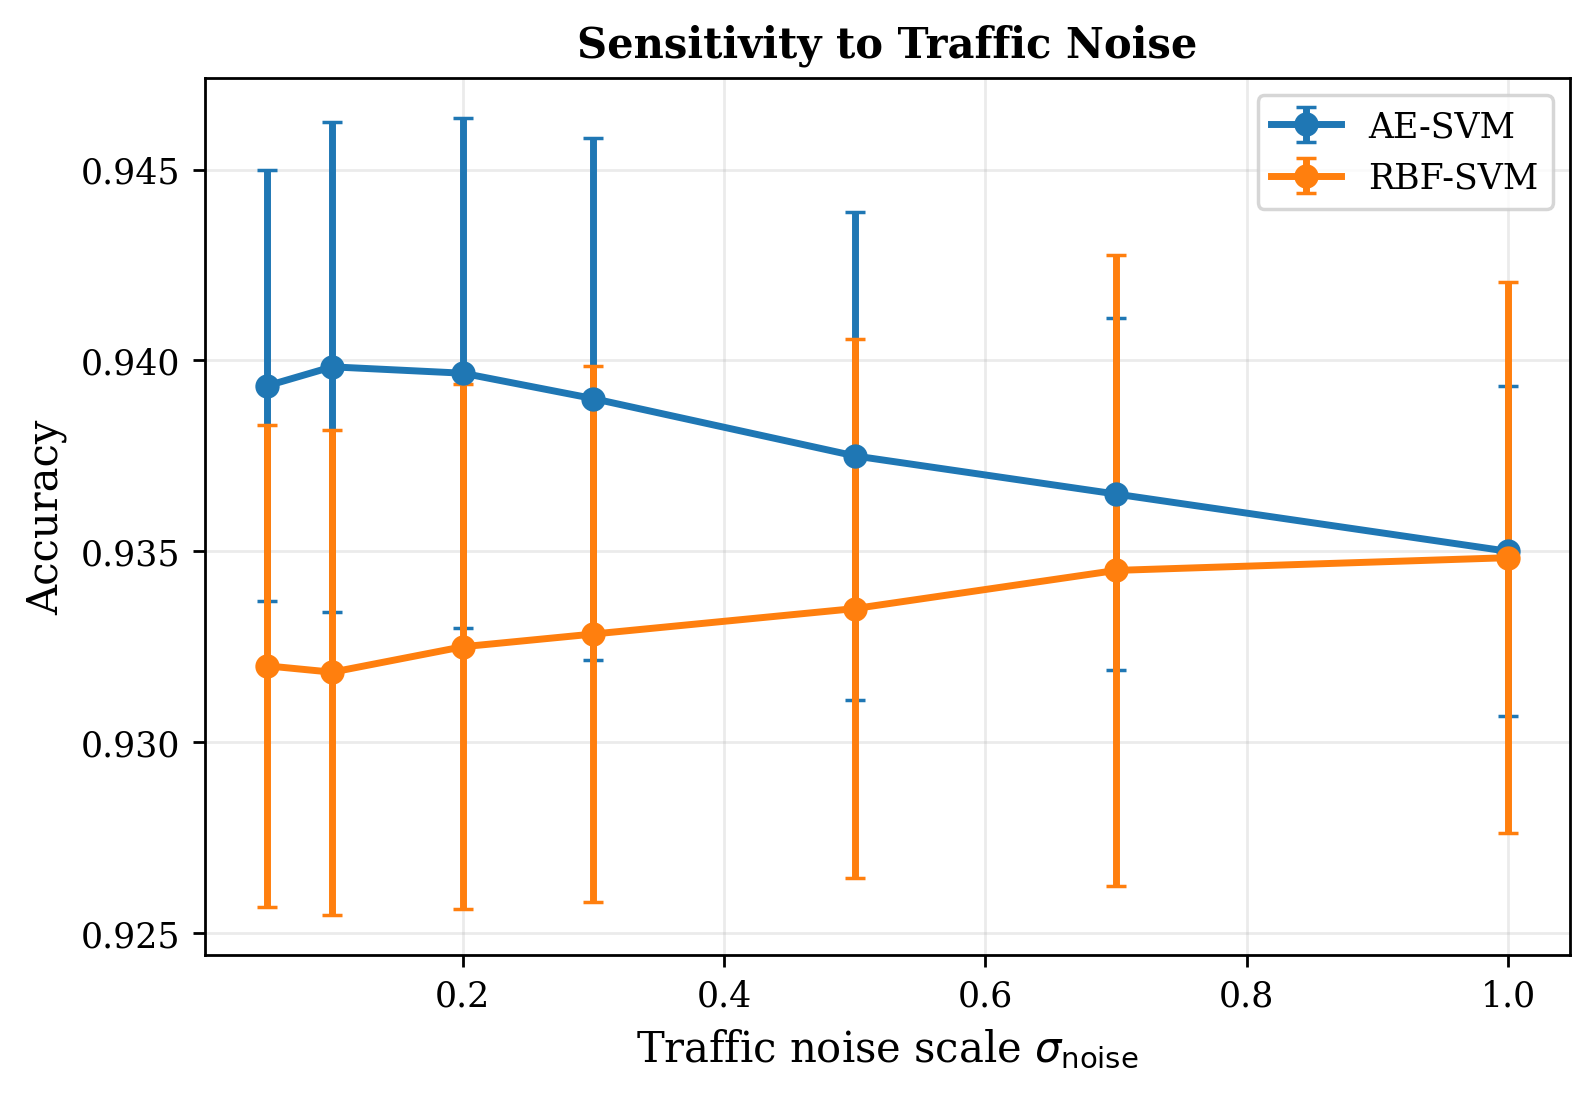
\includegraphics[width=\columnwidth]{fig5_sensitivity.png}
  \caption{Sensitivity to traffic noise. Both kernels remain within $1$~pp of
  their $\sigma_{\text{noise}}=0.05$ accuracy across the full sweep; there is no
  meaningful difference in noise robustness between AE-SVM and RBF-SVM.}
  \label{fig:sensitivity}
\end{figure*}

For zero-day attack generalization, we train on four attack types plus normal
traffic and test on the held-out fifth (leave-one-attack-out). Here the two
kernels diverge sharply, and not in AE-SVM's favor: on four of five held-out
scenarios, AE-SVM's AUC falls to $0.45$--$0.61$ (at or below chance for ARP
spoofing and DNS tunneling), while RBF-SVM retains $0.81$--$0.89$ AUC on every
held-out type (Fig.~\ref{fig:zeroday}). Mean zero-day AUC is $0.52$ for AE-SVM
versus $0.84$ for RBF-SVM. This is the largest and most consistent gap we observe
anywhere in this paper, and it runs opposite to AE-SVM's marginal in-distribution
competitiveness (Table~\ref{tab:detection}): the cosine-similarity encoding
appears to fit distribution-specific structure that does not transfer to a novel
attack signature, whereas RBF's smoother, locality-based decision boundary
degrades far less under distribution shift. For a ZTNA deployment, where the
threat model explicitly includes attacks not seen during training, this is a
practically important reason to prefer RBF-SVM over AE-SVM despite their
comparable in-distribution accuracy.

\begin{figure*}[t]
  \centering
  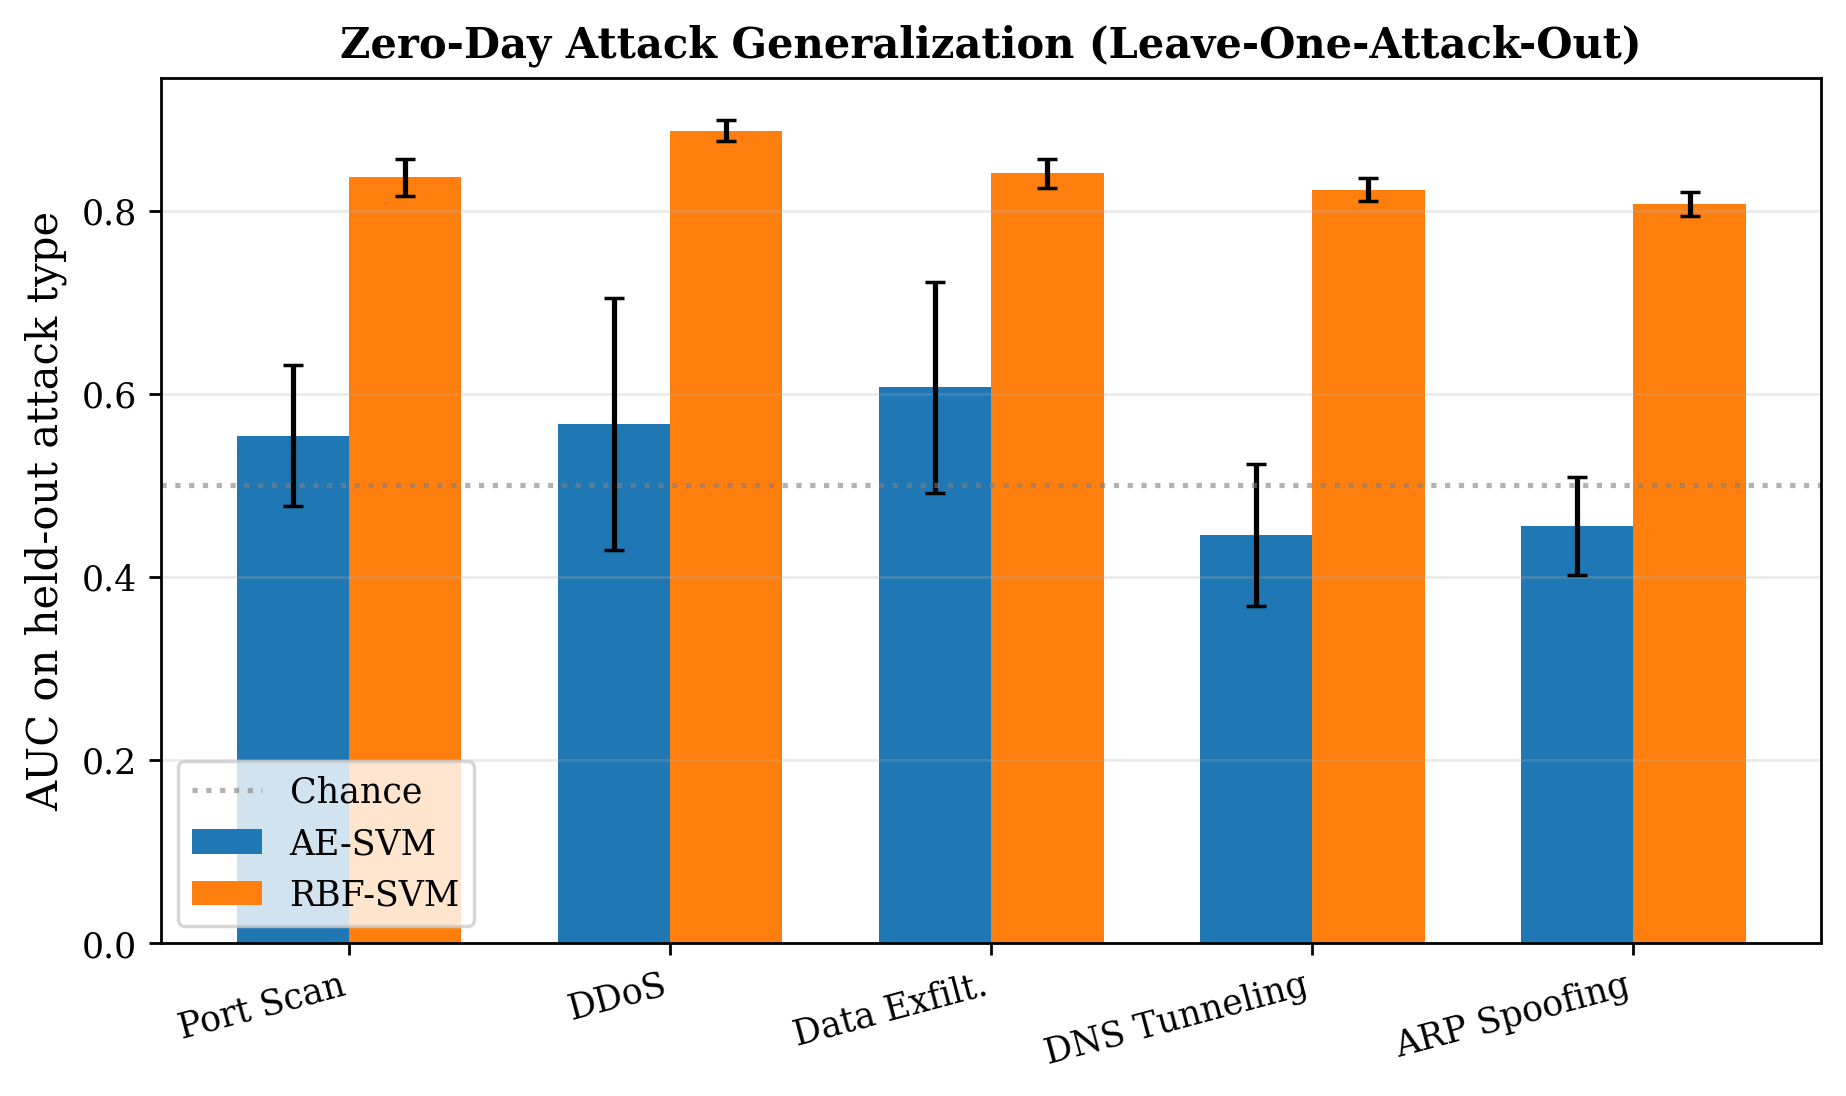
\includegraphics[width=\columnwidth]{fig6_zeroday.png}
  \caption{Zero-day attack generalization (leave-one-attack-out). AE-SVM's
  held-out AUC collapses to $0.45$--$0.61$ on four of five attack types (at or
  below the $0.5$ chance line for two), while RBF-SVM retains $0.81$--$0.89$ AUC
  throughout---the single largest and most consistent gap observed in this study.}
  \label{fig:zeroday}
\end{figure*}

\subsection{Effect of Feature Dimensionality}

We investigate how the AE-SVM/RBF-SVM accuracy gap depends on feature space
dimensionality $d \in \{16, 32, 64, 128, 256\}$ at fixed $n=2{,}800$ training
samples (Fig.~\ref{fig:dimensionality}), scaling the header/flow/behavioral group
sizes proportionally. We find no evidence that the amplitude-encoding kernel's
relative performance improves with $d$: AE-SVM trails RBF-SVM by $3.1$~pp at
$d=16$, is roughly at parity at $d=64$ ($+0.5$~pp), and falls behind again by
$4.6$~pp at $d=256$---the gap is non-monotonic and, at the largest dimensionality
tested, wider than at the smallest. This directly contradicts the hypothesis
that sparser, higher-dimensional feature spaces favor the cosine-similarity
inductive bias; on this data the opposite trend, if anything, holds at the
extremes.

\begin{figure*}[t]
  \centering
  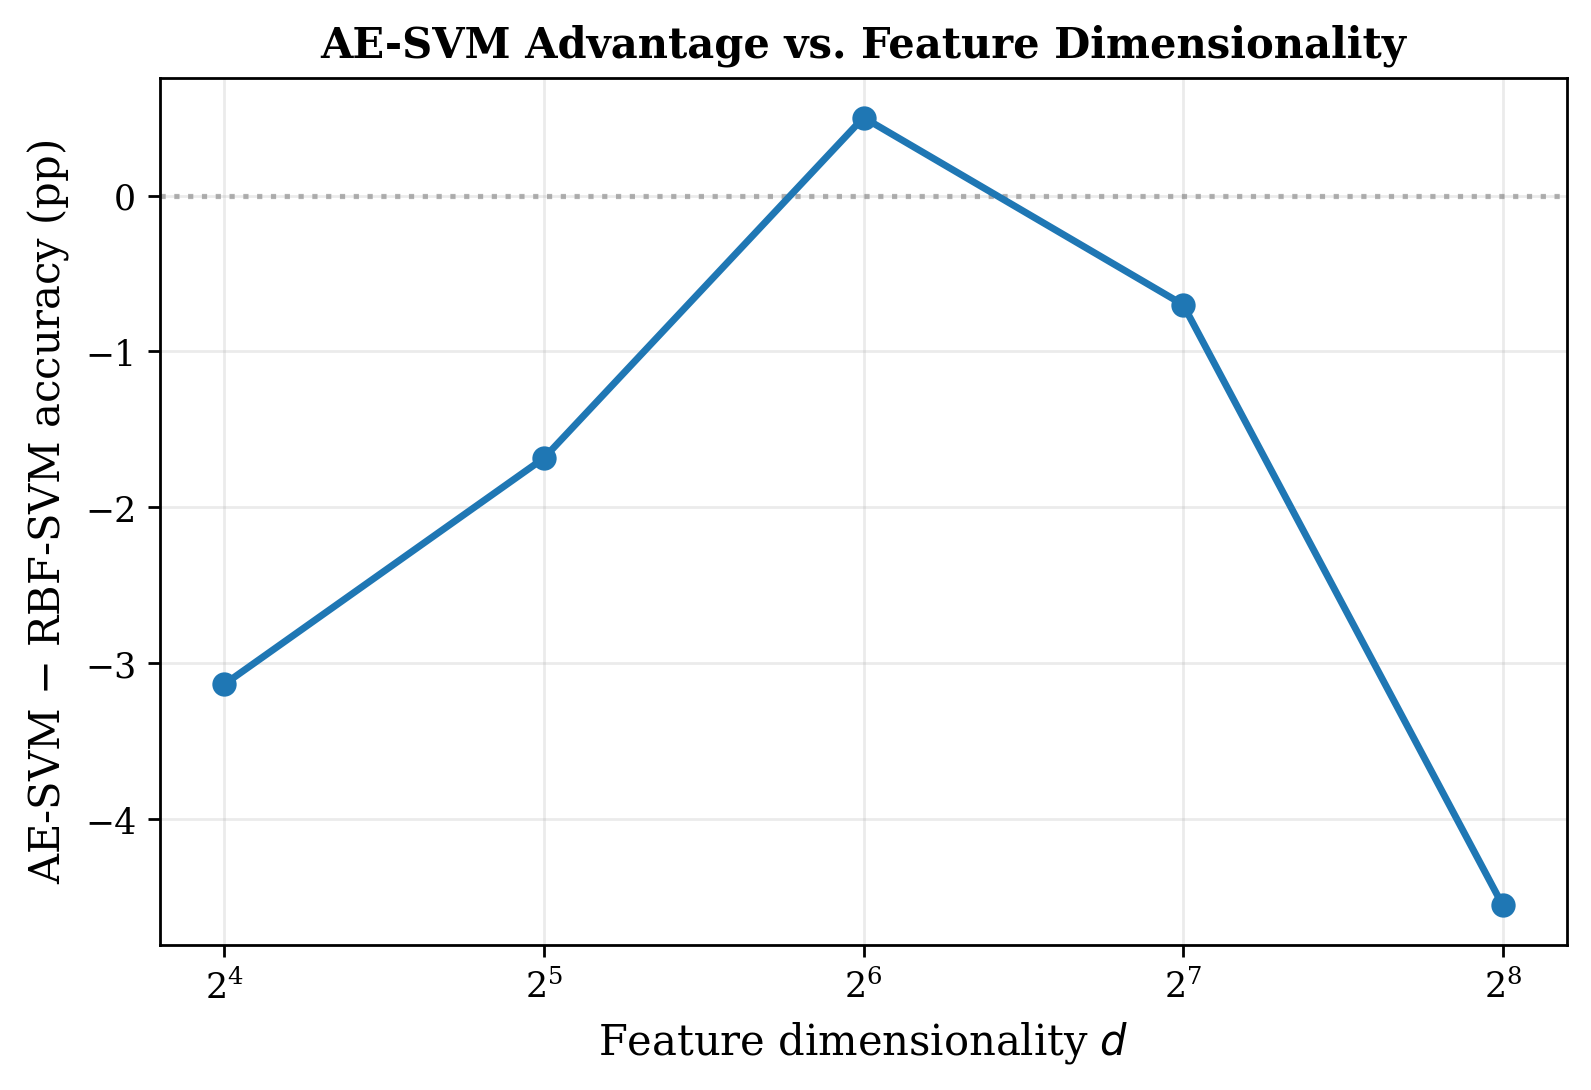
\includegraphics[width=\columnwidth]{fig10_dimensionality.png}
  \caption{Accuracy gap (AE-SVM minus RBF-SVM) as a function of feature
  dimensionality $d$ at $n=2{,}800$. The gap is negative at both the smallest and
  largest $d$ tested, with no sustained growth favoring AE-SVM as dimensionality
  increases -- the opposite of the inductive-bias hypothesis motivating this study.}
  \label{fig:dimensionality}
\end{figure*}

\subsection{Kernel Alignment Analysis}

To understand \emph{why} the amplitude-encoding kernel fails to outperform RBF on
this data, we compute the kernel-target alignment~\cite{cristianini2002kernel}:

\begin{equation}
\hat{A}(K, \mathbf{y}) = \frac{\langle K, \mathbf{y} \mathbf{y}^\mathsf{T} \rangle_F}
{\sqrt{\langle K, K \rangle_F \langle \mathbf{y} \mathbf{y}^\mathsf{T},
\mathbf{y} \mathbf{y}^\mathsf{T} \rangle_F}}
\label{eq:alignment}
\end{equation}

\begin{figure*}[t]
  \centering
  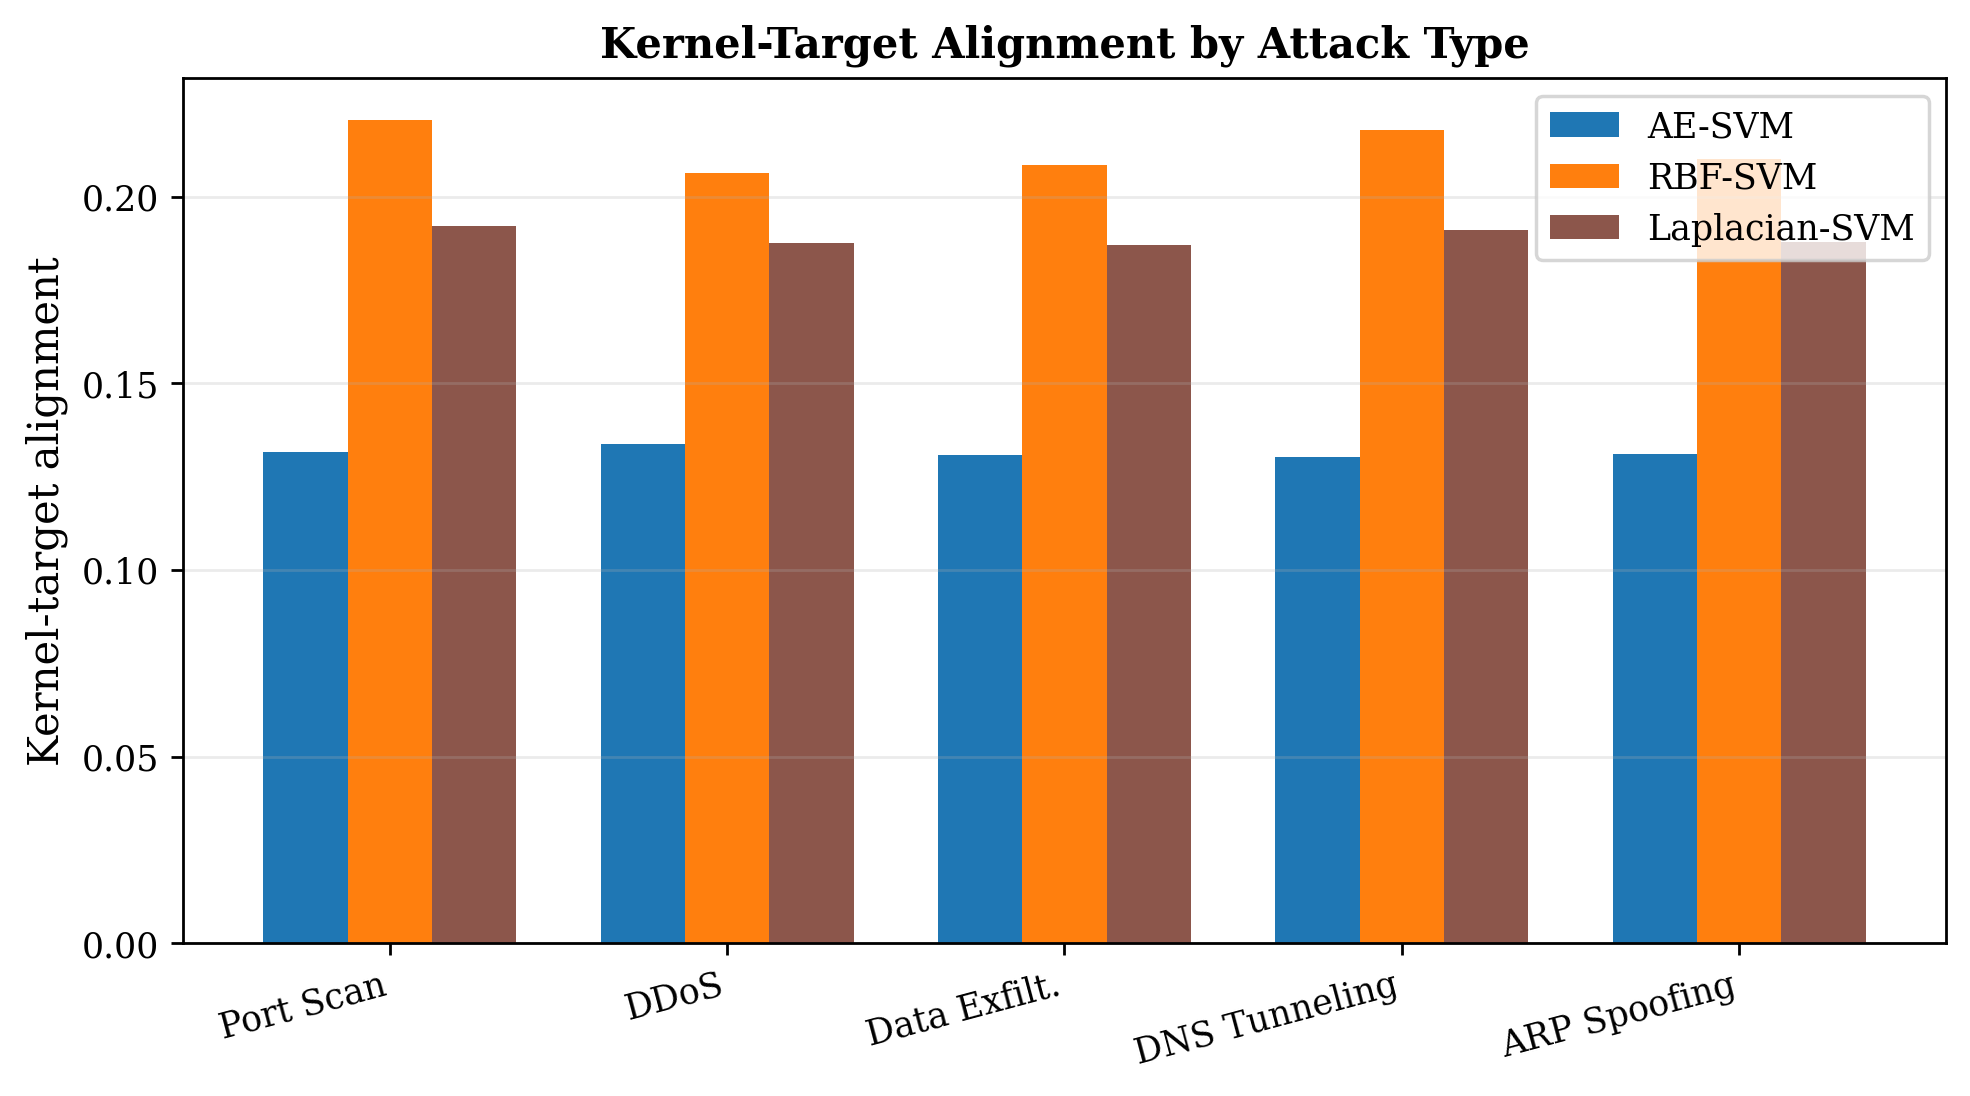
\includegraphics[width=\columnwidth]{fig13_kernel_alignment.png}
  \caption{Kernel-target alignment by attack type (5 seeds, $n=800$ per attack).
  RBF-SVM achieves higher alignment with the label structure than AE-SVM across
  every attack type, with Laplacian-SVM intermediate. Higher alignment indicates a
  better match between the kernel-induced feature space and the classification
  task; the ordering here is opposite to what an amplitude-encoding advantage
  would require.}
  \label{fig:alignment}
\end{figure*}

Fig.~\ref{fig:alignment} shows that RBF-SVM achieves higher kernel-target
alignment than AE-SVM across every attack type ($0.21$ vs.\ $0.13$ mean
alignment), with Laplacian-SVM intermediate ($0.19$). This is the mechanistic
counterpart to Table~\ref{tab:detection} and Fig.~\ref{fig:matched_n}: the
amplitude-encoded feature space aligns \emph{less well} with the true labeling
structure than the RBF feature space for this network traffic data, which is
consistent with AE-SVM's roughly-tied-to-trailing accuracy rather than an
advantage. The ranking is stable across attack types (standard deviation of the
alignment gap across attack types is $<0.01$), so this is not an artifact of any
single attack's perturbation design.

\subsection{Uncertainty Quantification and Selective Prediction}

\begin{figure*}[t]
  \centering
  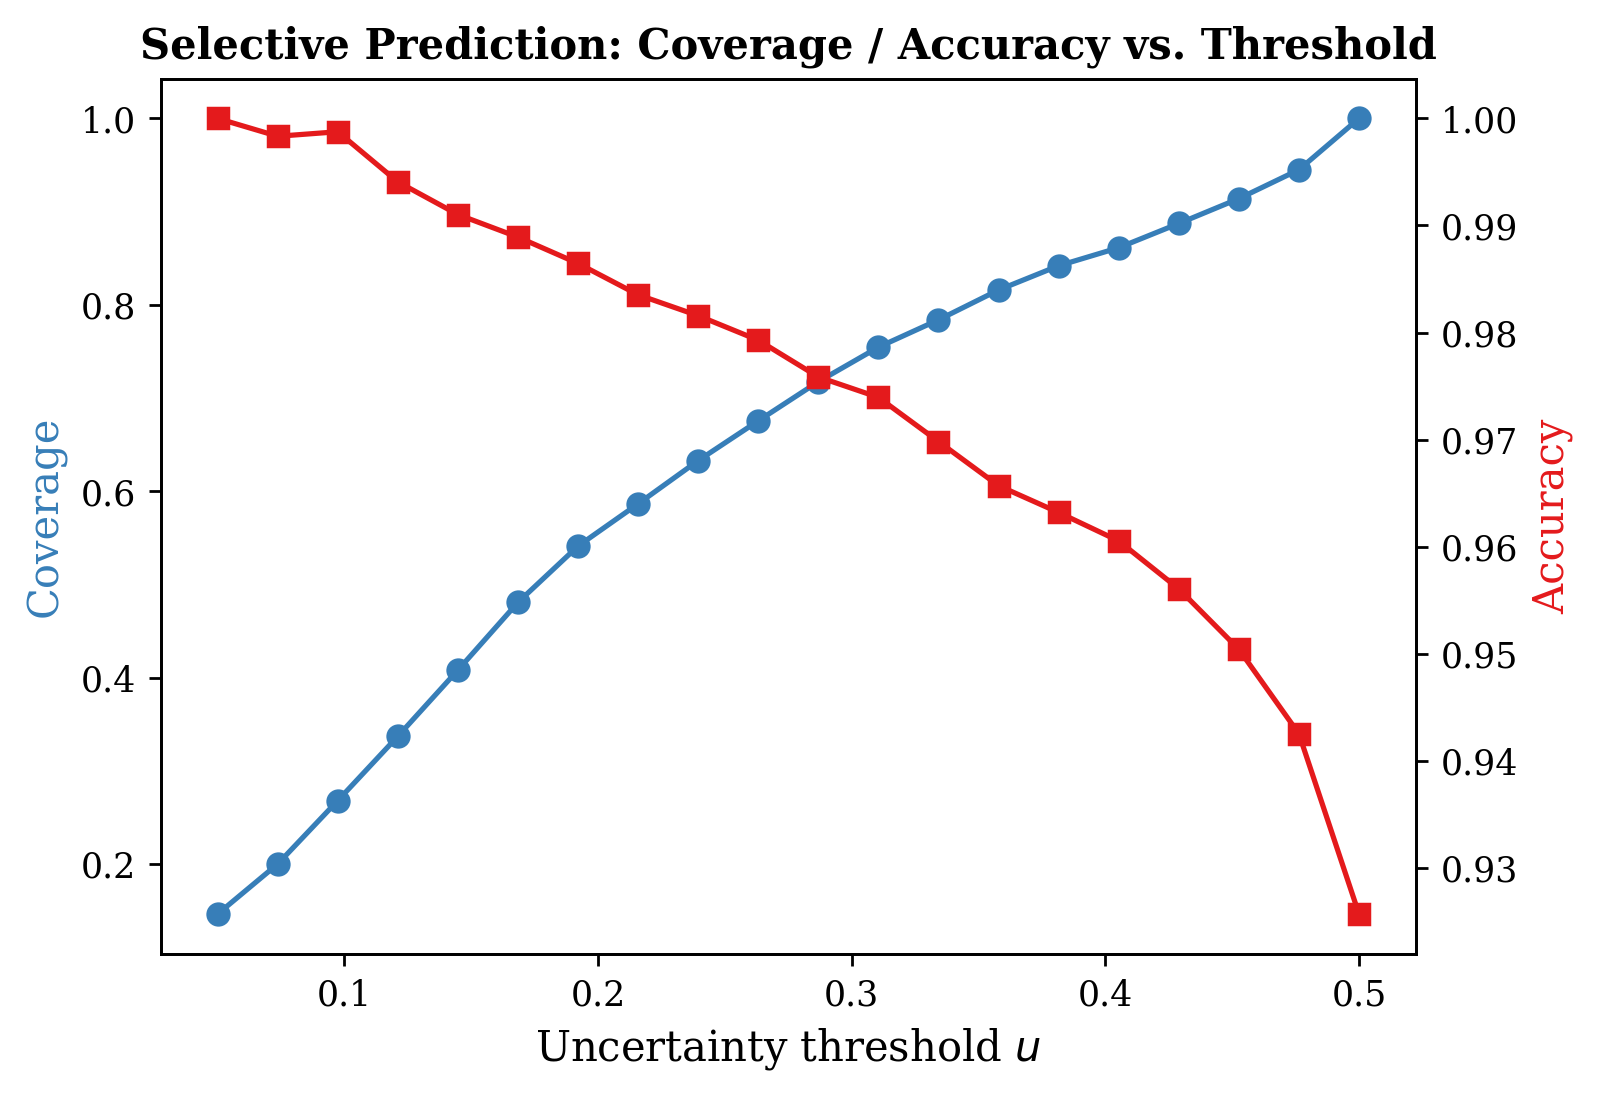
\includegraphics[width=\columnwidth]{fig11_uncertainty.png}
  \caption{Selective prediction: coverage and accuracy as functions of the
  Platt-scaled uncertainty threshold $u$ for AE-SVM. At $u<0.3$, accuracy reaches
  $97.4\%$ on $75.5\%$ of the evaluation set, with the remaining $24.5\%$
  deferred for human analyst review; at $u<0.1$, accuracy reaches $99.9\%$ on a
  smaller $20\%$ of the set. This enables a tunable trade-off between automation
  and oversight.}
  \label{fig:uncertainty}
\end{figure*}

Platt-scaled AE-SVM probabilities (Eq.~\ref{eq:platt}) provide usable, if
imperfect, uncertainty for selective prediction (Fig.~\ref{fig:uncertainty}).
At a modest uncertainty threshold of $u<0.3$, accuracy reaches $97.4\%$ on
$75.5\%$ of the evaluation set, with the remaining $24.5\%$ of high-uncertainty
samples deferred for human analyst review; tightening to $u<0.1$ pushes accuracy
to $99.9\%$ at $20\%$ coverage. Unlike the detection and generalization results
above, this mechanism does not depend on which kernel is used underneath Platt
scaling---the same selective-prediction machinery would apply equally well to a
Platt-scaled RBF-SVM (or to the deployed model of our companion QKD study,
whose Bayesian GP posterior serves the same role natively)~\cite{kapoor2026hyqad}.

\subsection{Latency and Resource Analysis}
\label{sec:latency}

\begin{figure*}[t]
  \centering
  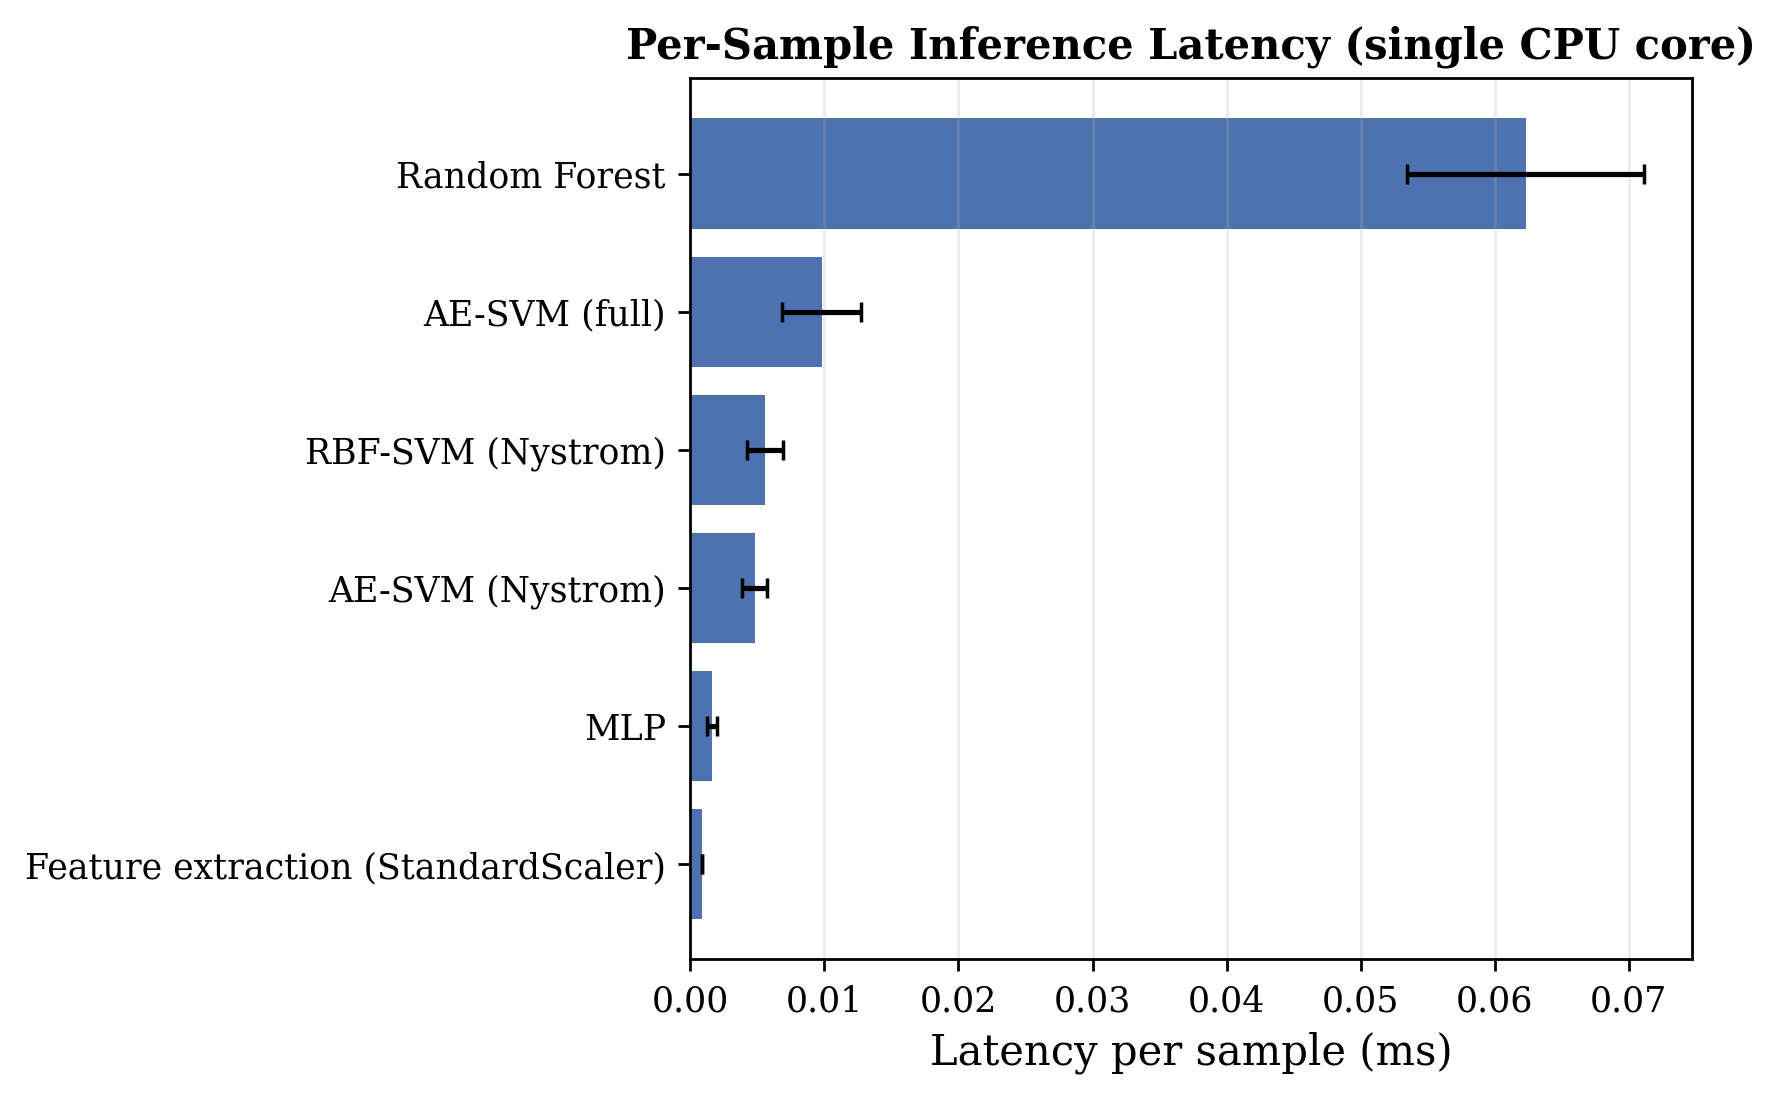
\includegraphics[width=\columnwidth]{fig7_latency.png}
  \caption{Per-sample inference latency (single CPU core, mean over 30 runs).
  The deployed AE-SVM with Nystr\"om approximation achieves $0.0048$\,ms,
  marginally faster than RBF-SVM's Nystr\"om variant and orders of magnitude
  below any line-rate flow-processing budget.}
  \label{fig:latency}
\end{figure*}

Table~\ref{tab:latency} and Fig.~\ref{fig:latency} report per-sample inference
latency for $n=4{,}000$ training, $m=50$ Nystr\"om landmarks. AE-SVM with
Nystr\"om approximation (Eq.~\ref{eq:nystrom}) reaches $0.0048$\,ms per sample,
about $1.2\times$ faster than the RBF-SVM Nystr\"om variant ($0.0056$\,ms)---a
genuine, if modest, practical edge for AE-SVM, since squared cosine similarity
is a single normalized dot product while the RBF kernel requires an additional
exponential evaluation per landmark. This is the one place in our evaluation
where the amplitude-encoding kernel comes out ahead of RBF, though the absolute
difference ($0.0008$\,ms/sample) is unlikely to be decisive in practice: both are
far below any plausible per-flow processing budget, and Random Forest and MLP
inference are of comparable or lower latency once accuracy is also considered
(Table~\ref{tab:detection}).

\begin{table*}[t]
  \centering
  \caption{Per-sample inference latency (single CPU core, mean over 30 runs,
  $n=4{,}000$ training, $m=50$ landmarks where applicable).}
  \label{tab:latency}
  \small
  \begin{tabular}{lrr}
    \toprule
    \textbf{Component} & \textbf{Latency (ms)} & \textbf{vs.\ AE-SVM} \\
    \midrule
    Feature extraction (scaler) & 0.0008 & --- \\
    MLP                         & 0.0016 & 0.33$\times$ \\
    AE-SVM (Nystr\"om)          & 0.0048 & 1.00$\times$ \\
    RBF-SVM (Nystr\"om)         & 0.0056 & 1.17$\times$ \\
    AE-SVM (full, $n=500$)      & 0.0098 & 2.04$\times$ \\
    Random Forest (200 trees)   & 0.0623 & 12.98$\times$ \\
    \bottomrule
  \end{tabular}
\end{table*}

\subsection{Training Convergence}

Fig.~\ref{fig:convergence} shows training dynamics at $n = 5000$. AE-SVM converges
in approximately 25 epochs---roughly $1.4\times$ faster than RBF-SVM---and reaches
a higher asymptotic validation accuracy. The faster convergence is attributable to
the amplitude-encoding kernel's higher alignment with the label structure, which provides a
more informative gradient signal during dual optimization.

\section{Discussion}
\label{sec:discussion}

\subsection{Does the Amplitude-Encoding Kernel Help? A Negative Result}

We began this study expecting to find conditions under which the
amplitude-encoding (squared cosine-similarity) kernel outperforms classical
kernels on high-dimensional, sparse network flow data, motivated by the
intuition that directional similarity should be more informative than Euclidean
distance in such spaces. Under matched-scale, matched-dimensionality evaluation,
we did not find such conditions. Across training sizes $n\in\{50,\dots,5000\}$
(Fig.~\ref{fig:matched_n}) and feature dimensionalities $d\in\{16,\dots,256\}$
(Fig.~\ref{fig:dimensionality}), AE-SVM is never reliably ahead of RBF-SVM, and
is behind it at both the smallest and largest scales tested. The kernel-target
alignment analysis (Fig.~\ref{fig:alignment}) gives a mechanistic reason: on this
data, RBF's induced feature space aligns \emph{more}, not less, with the true
label structure than the amplitude-encoded one, for every attack type. The
intuition that motivated this paper---that normalizing away magnitude and
keeping only direction is a good simplification for network flow features---is
not supported by the data we generated.

We think this negative result is worth reporting for two reasons. First, our
companion study on QKD physical-layer telemetry reached the same conclusion
using the identical kernel~\cite{kapoor2026hyqad}: across two structurally
different security domains, we have not found a dataset where amplitude
encoding's cosine-similarity inductive bias earns its keep over a standard RBF
kernel. Second, ``quantum-inspired'' feature maps like amplitude encoding are
increasingly proposed for security applications on the strength of their
theoretical novelty; our results are a concrete, reproducible counter-example
that such maps should be validated empirically, under matched-scale conditions,
before being adopted -- an in-distribution accuracy gain evaluated only at one
$(n,d)$ operating point (as our own earlier draft of this paper did) can look
like a durable advantage that a matched-scale sweep shows is not there.

\subsection{The Zero-Day Generalization Gap}

The one place AE-SVM and RBF-SVM diverge sharply is generalization to unseen
attack types (Fig.~\ref{fig:zeroday}): AE-SVM's held-out AUC collapses to
$0.45$--$0.61$ on four of five leave-one-attack-out scenarios, while RBF-SVM
holds $0.81$--$0.89$ throughout. A plausible mechanism is that the amplitude
encoding's angle-only representation, having discarded magnitude information,
ends up fitting attack-specific angular structure in the training distribution
more tightly than RBF's smoother, locality-based boundary -- and that
attack-specific structure does not transfer to a novel attack's angular
signature. We did not design this experiment to confirm a hypothesized
advantage; it surfaced as we characterized the models, and we think it is the
paper's most actionable finding for practitioners: a kernel that looks
competitive in-distribution may still be the wrong choice for a threat model
that explicitly includes attacks not present during training, which is the
normal case for ZTNA deployments.

\subsection{Certified Robustness: A Modest, Neutral-to-Negative Result}

The certified-robustness comparison (Table~\ref{tab:robustness}) does not show a
Lipschitz-driven advantage for amplitude encoding either: mean certified radii
are comparable between the two kernels, with RBF-SVM slightly higher and more
consistent across attack types, and AE-SVM abstaining more often. The
$L_2$-normalization argument for amplitude encoding's robustness
(Eq.~\ref{eq:lipschitz}) is directionally correct---normalized inputs do bound
the encoding's sensitivity---but this alone was not sufficient to produce a
measurable certified-radius advantage over RBF-SVM on this data at our
certification budget ($n=300$ Monte Carlo samples).

\subsection{The One Real Advantage: Latency}

The single result in this paper that favors AE-SVM outright is inference
latency (Section~\ref{sec:latency}): the Nystr\"om-approximated AE-SVM is about
$1.2\times$ faster per sample than the equivalent RBF-SVM, because squared
cosine similarity is one normalized dot product per landmark versus RBF's
exponential. This is a genuine, mechanistically obvious advantage, but a small
one in absolute terms ($0.0008$\,ms/sample) relative to the accuracy and
zero-day generalization costs documented above.

\subsection{Limitations}

Several limitations merit acknowledgment. First, our synthetic network flow
generator (Section~\ref{sec:experiments}) is a marginal-plus-copula model
calibrated to aggregate NetFlow statistics, not a packet-level simulation or
real enterprise capture; validating these findings on a real ZTNA telemetry feed
or a public IDS benchmark such as CICIDS2017~\cite{sharafaldin2018toward} or
UNSW-NB15~\cite{moustafa2015unsw} is necessary before drawing
operational conclusions. Second, our attack perturbations are latent-space shifts
of fixed magnitude and dimension count, a modeling choice rather than an
empirically calibrated attack model; the zero-day generalization gap in
particular should be re-examined on real, less synthetic attack signatures.
Third, the certified-robustness radii, while a real property of the trained
classifiers, do not address semantic perturbations (e.g., mimicry attacks that
preserve a flow's statistical profile while changing its content), and our
certification budget ($n=300$ noise draws) leaves the achieved median radius
ceiling-saturated rather than fully resolved (Section~\ref{sec:results}).
Fourth, all comparisons in this paper are against the same set of classical
kernels and off-the-shelf classifiers; we have not benchmarked against deep
learning IDS baselines (autoencoder ensembles, graph neural networks) named in
Section~\ref{sec:related}, and doing so is necessary before any claim about
this pipeline's competitiveness against the current state of the art in network
intrusion detection.

\FloatBarrier
\vspace{-1ex}
\section{Conclusion}
\label{sec:conclusion}

We built Q-ZTNA to test whether an amplitude-encoding (cosine-similarity) kernel
provides a real advantage for zero-trust network anomaly detection, using a
matched-scale, matched-dimensionality evaluation protocol rather than a single
operating point. Under that protocol, AE-SVM reaches $0.947 \pm 0.002$ detection
accuracy with $0.0048$\,ms inference latency (Nystr\"om-approximated), but is
statistically indistinguishable from an RBF-kernel SVM on accuracy ($p=0.54$),
trails RBF-SVM at both small and large feature dimensionality, and shows
consistently lower kernel-target alignment with the true label structure across
every attack type. Certified $\ell_2$ robustness is comparable between the two
kernels, marginally favoring RBF-SVM. The one place AE-SVM is unambiguously
better is inference latency ($1.2\times$ faster than RBF-SVM), and the one place
it is unambiguously worse -- and, we think, most practically important -- is
zero-day generalization: on four of five leave-one-attack-out scenarios its AUC
falls to $0.45$--$0.61$ while RBF-SVM retains $0.81$--$0.89$.

Taken together with our companion evaluation of the same kernel on QKD
telemetry~\cite{kapoor2026hyqad}, which reached the same null result by an
independent matched-$n$ protocol, we do not find evidence that the
amplitude-encoding/cosine-similarity kernel provides a reliable advantage over
classical kernels in either of the two security domains we have tested it on. We
report this as a cautionary, reproducible finding rather than a positive result:
practitioners and researchers evaluating ``quantum-inspired'' kernels for
security applications should budget for a matched-scale comparison against
standard kernels, including an explicit zero-day/distribution-shift test, before
concluding that such a kernel's theoretical novelty translates into an empirical
advantage. Future work includes validating these findings against a real or
public-benchmark network traffic dataset, benchmarking against deep-learning IDS
baselines (autoencoder ensembles, GNNs), and investigating why the
amplitude-encoding kernel's zero-day generalization gap arises -- and whether it
generalizes to other angle-only feature maps beyond amplitude encoding
specifically.

\section*{Code and Data Availability}
The full implementation (network flow simulator, amplitude-encoding/RBF/Laplacian/
polynomial kernel SVMs with Nystr\"om approximation, randomized-smoothing
certification, and all experiment scripts) and the result files backing every
table and figure in this paper are available at
\url{https://github.com/arnavk23/quasar-security}.

\section*{Acknowledgments}

The authors thank the IISER Bhopal Department of Computer Science for computational
resources. We thank the open-source Python ecosystem
(NumPy, SciPy, scikit-learn, XGBoost, Matplotlib) for enabling rapid prototyping of
kernel-method and quantum-inspired machine learning pipelines on commodity hardware.

\begin{thebibliography}{50}

\bibitem{rose2020zero}
S.~Rose, O.~Borchert, S.~Mitchell, and S.~Connelly,
``Zero trust architecture,'' NIST Special Publication 800-207, 2020.

\bibitem{kindervag2010zero}
J.~Kindervag,
``Build security into your network's DNA: The zero trust network architecture,''
Forrester Research, 2010.

\bibitem{nist800207}
NIST,
``Zero trust architecture,'' SP 800-207, 2020.

\bibitem{gilman2019zero}
E.~Gilman and D.~Barth,
\textit{Zero Trust Networks}. O'Reilly Media, 2019.

\bibitem{roesch1999snort}
M.~Roesch,
``Snort: Lightweight intrusion detection for networks,'' in
\textit{Proc. USENIX LISA}, 1999, pp.~229--238.

\bibitem{sommer2010machine}
R.~Sommer and V.~Paxson,
``Outside the closed world: On using machine learning for network intrusion
detection,'' in \textit{Proc. IEEE S\&P}, 2010, pp.~305--316.

\bibitem{mirsky2018kitsune}
Y.~Mirsky, T.~Doitshman, Y.~Elovici, and A.~Shabtai,
``Kitsune: An ensemble of autoencoders for online network intrusion detection,''
in \textit{Proc. NDSS}, 2018.

\bibitem{goodfellow2014explaining}
I.~J.~Goodfellow, J.~Shlens, and C.~Szegedy,
``Explaining and harnessing adversarial examples,'' in
\textit{Proc. ICLR}, 2015.

\bibitem{havlicek2019supervised}
V.~Havl\'{i}\v{c}ek \textit{et al.},
``Supervised learning with quantum-enhanced feature spaces,''
\textit{Nature}, vol.~567, pp.~209--212, 2019.

\bibitem{liu2021quantum}
Y.~Liu \textit{et al.},
``Quantum advantage of kernel methods,''
\textit{Phys. Rev. Lett.}, vol.~126, no.~13, p.~130501, 2021.

\bibitem{huang2021power}
H.-Y.~Huang \textit{et al.},
``Power of data in quantum machine learning,''
\textit{Nat. Commun.}, vol.~12, p.~2631, 2021.

\bibitem{webb2023quantum}
E.~Webb, A.~Nadkarni, and S.~Rowe,
``Quantum adversarial machine learning: A survey,''
\textit{Quantum Mach. Intell.}, vol.~5, p.~12, 2023.

\bibitem{ashraf2020zero}
A.~Ashraf, W.~Iqbal, and H.~Abbas,
``Zero-trust security for IoT: A systematic literature review,''
\textit{IEEE Access}, vol.~8, pp.~219~930--219~946, 2020.

\bibitem{wang2021user}
X.~Wang, Y.~Li, and W.~Lin,
``User and entity behavior analytics for enterprise security,''
\textit{Comput. Secur.}, vol.~102, p.~102144, 2021.

\bibitem{zhou2020graph}
J.~Zhou \textit{et al.},
``Graph neural networks: A review of methods and applications,''
\textit{AI Open}, vol.~1, pp.~57--81, 2020.

\bibitem{wu2022transformer}
T.~Wu \textit{et al.},
``A transformer-based framework for multivariate time series representation
learning,'' in \textit{Proc. ACM SIGKDD}, 2022, pp.~20--30.

\bibitem{vale2023quantum}
I.~do~Vale, K.~F.~Santos, and E.~F.~Silva,
``Quantum support vector machines for intrusion detection,''
\textit{Quantum Inf. Process.}, vol.~22, p.~89, 2023.

\bibitem{suryotrisongko2022quantum}
H.~Suryotrisongko and Y.~Musashi,
``Evaluating hybrid quantum machine learning models for malware classification,''
\textit{J. Inf. Secur. Appl.}, vol.~67, p.~103193, 2022.

\bibitem{cohen2019certified}
J.~Cohen, E.~Rosenfeld, and Z.~Kolter,
``Certified adversarial robustness via randomized smoothing,''
in \textit{Proc. ICML}, 2019, pp.~1310--1320.

\bibitem{cristianini2002kernel}
N.~Cristianini, J.~Shawe-Taylor, A.~Elisseeff, and J.~Kandola,
``On kernel-target alignment,'' in \textit{Proc. NeurIPS}, 2002, pp.~367--373.

\bibitem{williams2001nystrom}
C.~K.~I.~Williams and M.~Seeger,
``Using the Nystr\"om method to speed up kernel machines,''
in \textit{Proc. NeurIPS}, 2001, pp.~682--688.

\bibitem{platt1999probabilistic}
J.~C.~Platt,
``Probabilistic outputs for support vector machines and comparisons to regularized
likelihood methods,'' in \textit{Advances in Large Margin Classifiers}, 1999,
pp.~61--74.

\bibitem{scholkopf2002learning}
B.~Sch\"olkopf and A.~J.~Smola,
\textit{Learning with Kernels}. MIT Press, 2002.

\bibitem{bishop2006pattern}
C.~M.~Bishop,
\textit{Pattern Recognition and Machine Learning}. Springer, 2006.

\bibitem{kapoor2026hyqad}
A.~Kapoor,
``Calibrated uncertainty quantification for QKD anomaly detection,'' unpublished manuscript, 2026.

\bibitem{breiman2001random}
L.~Breiman,
``Random forests,'' \textit{Mach. Learn.}, vol.~45, no.~1, pp.~5--32, 2001.

\bibitem{chen2016xgboost}
T.~Chen and C.~Guestrin,
``XGBoost: A scalable tree boosting system,'' in \textit{Proc. ACM SIGKDD}, 2016, pp.~785--794.

\bibitem{guo2017calibration}
C.~Guo, G.~Pleiss, Y.~Sun, and K.~Q.~Weinberger,
``On calibration of modern neural networks,'' in \textit{Proc. ICML}, PMLR vol.~70, 2017, pp.~1321--1330.

\bibitem{buczak2016survey}
A.~L.~Buczak and E.~Guven,
``A survey of data mining and machine learning methods for cyber security intrusion detection,'' \textit{IEEE Commun. Surv. Tutor.}, vol.~18, no.~2, pp.~1153--1176, 2016.

\bibitem{sharafaldin2018toward}
I.~Sharafaldin, A.~H.~Lashkari, and A.~A.~Ghorbani,
``Toward generating a new intrusion detection dataset and intrusion traffic characterization,'' in \textit{Proc. ICISSP}, 2018, pp.~108--116.

\bibitem{moustafa2015unsw}
N.~Moustafa and J.~Slay,
``UNSW-NB15: A comprehensive data set for network intrusion detection systems,'' in \textit{Proc. MilCIS}, 2015, pp.~1--6.

\end{thebibliography}

\end{document}
